\documentclass[a4paper,UKenglish,cleveref,autoref,anonymous,numberwithinsect]{lipics-v2021}

\usepackage[ruled,vlined,linesnumbered]{algorithm2e}
\AtBeginDocument{\DontPrintSemicolon}
\usepackage{tikz}
\usetikzlibrary{shapes.geometric}
\usepackage{pgfplots}
\pgfplotsset{compat=1.18}
\usepackage{capt-of}
\usepackage{float}
\SetArgSty{textnormal}

% Define colors
\definecolor{cutA}{RGB}{214,39,40}
\definecolor{cutB}{RGB}{31,119,180}
\definecolor{cutC}{RGB}{44,160,44}
\definecolor{cutD}{RGB}{23,190,207}
\definecolor{cutE}{RGB}{148,103,189}
\definecolor{cutF}{RGB}{140,86,75}

% Bracket and notation macros
\newcommand{\br}[1]{\mathopen{}\left( #1 \right)}
\newcommand{\brc}[1]{\mathopen{}\left\{ #1 \right\}}
\newcommand{\spr}[1]{\mathopen{}\left| #1 \right|}
\newcommand{\fl}[1]{\mathopen{}\left\lfloor #1 \right\rfloor}
\newcommand{\cl}[1]{\mathopen{}\left\lceil #1 \right\rceil}
\newcommand{\angl}[1]{\mathopen{}\langle #1 \rangle}
\newcommand{\e}[1]{\exp\left\{ #1 \right\}}

% Algorithm and notation
\newcommand{\Cent}{\texttt{Cent}}
\newcommand{\APP}{\texttt{APP}}
\newcommand{\DPartition}{\textsc{DPartition}}
\newcommand{\cut}{\delta}
\newcommand{\Etree}{\mathbb{E}_{T\sim\mu}}
\newcommand{\DD}[1]{\textcolor{red}{DD: #1}}
\newcommand{\DDfix}[1]{\textcolor{violet}{#1}}
\newcommand{\bigo}{\mathcal{O}}
\newcommand{\minCut}[3]{\textup{min-cut}_{#3}\br{#1,#2}}
\newcommand{\phiwK}{\phi_w^{K}}
\newcommand{\OPTh}{\OPT_h^{\delta}}
\newcommand{\OPTc}{\OPT_{\psi}}
\newcommand{\OPTdem}[2]{\OPT_{#2}\br{#1}}
\newcommand{\paths}{P^*}
\newcommand{\OPT}{\textup{OPT}}
\DeclareMathOperator*{\argmin}{arg\,min}
\DeclareMathOperator*{\argmax}{arg\,max}
\newcommand{\cov}{\text{cov}}
\newcommand{\ct}{\text{ct}}
\newcommand{\Sopt}{S_h^{*}}
\newcommand{\SoptBar}{\bar{S}_h^{*}}
\newcommand{\hw}{h_w^{\delta}}
\newcommand{\hOPT}{S_h^{\delta}(G)}
\newcommand{\psiOPT}{S_{\psi}(G)}
\newcommand{\COST}{{c}}
\newcommand{\dist}{\text{dist}}
\newcommand{\ch}{\text{ch}}
\newcommand{\supp}{\operatorname{supp}}
\newcommand{\vol}{\operatorname{vol}}
\newcommand{\lca}{\operatorname{lca}}

% Calligraphic letter macros
\newcommand{\cA}{\mathcal{A}}
\newcommand{\cB}{\mathcal{B}}
\newcommand{\cC}{\mathcal{C}}
\newcommand{\cD}{\mathcal{D}}
\newcommand{\cE}{\mathcal{E}}
\newcommand{\cF}{\mathcal{F}}
\newcommand{\cG}{\mathcal{G}}
\newcommand{\cH}{\mathcal{H}}
\newcommand{\cI}{\mathcal{I}}
\newcommand{\cJ}{\mathcal{J}}
\newcommand{\cK}{\mathcal{K}}
\newcommand{\cL}{\mathcal{L}}
\newcommand{\cM}{\mathcal{M}}
\newcommand{\cN}{\mathcal{N}}
\newcommand{\cO}{\mathcal{O}}
\newcommand{\cP}{\mathcal{P}}
\newcommand{\cQ}{\mathcal{Q}}
\newcommand{\cR}{\mathcal{R}}
\newcommand{\cS}{\mathcal{S}}
\newcommand{\cT}{\mathcal{T}}
\newcommand{\cU}{\mathcal{U}}
\newcommand{\cV}{\mathcal{V}}
\newcommand{\cW}{\mathcal{W}}
\newcommand{\cX}{\mathcal{X}}
\newcommand{\cY}{\mathcal{Y}}
\newcommand{\cZ}{\mathcal{Z}}


\title{Graph Partitioning with Demands: Generalized Conductance and its Applications}
\titlerunning{Graph Partitioning with Demands}

\author{Anonymous Author(s)}{Anonymous Institution, Anonymous City, Anonymous Country}{}{}{}
\authorrunning{Anonymous Authors}
\Copyright{Anonymous Authors}

\ccsdesc[500]{Theory of computation~Design and analysis of algorithms}
\keywords{Graph partitioning with demands, Generalized conductance, Sparsest cut, Hierarchical clustering, Approximation algorithms}

\bibliographystyle{plainurl}

\begin{document}

\maketitle

\begin{abstract}
We study various graph partitioning tasks subject to general partitioning demands. In \textsc{Graph Partitioning with Demands} (GPD), the goal is to delete supply edges of minimum total cost so that each remaining component contains at most a prescribed fraction of the total demand. In \textsc{Hierarchical Clustering with Demands} (HCD), the goal is to build a hierarchy of clusters, charging each supply edge by the demand in the smallest cluster containing its endpoints.

Our main general-graph results are approximation algorithms for GPD and HCD. For every fixed $0<\rho<\eta<1$, we give a polynomial-time bicriteria algorithm for GPD whose components have demand at most $\eta \cdot W$ and whose cost is at most $\mathcal{O}_{\rho,\eta}(\sqrt{\log n})$ times the optimum cost for threshold $\rho$. This algorithm can be then recursively used to obtain an $\mathcal{O}(\sqrt{\log n})$-approximation for HCD. The algorithm for GPD itself iteratively uses a crucial subproblem called \textsc{Generalized Conductance} (GC), which is a new generalization of the unit-demand sparsest cut. The latter is then reducible to the well-known \textsc{Min-Ratio Vertex Cut} problem.

On supply trees, we show that GC can be solved exactly in polynomial time, which leads to improved algorithms for GPD and HCD on trees. We also give bicriteria algorithms for GPD based on anchored-LP rounding and separator recursion, as well as a single-criterion $(4+\epsilon)$-approximation in $n^{O(1/\rho)}$ time. The GPD algorithms yield a $\frac{4e}{e-1}$-approximation for HCD on trees. \textsc{Generalized Conductance} is NP-hard to approximate within any constant factor, even with unit demand on every pair of vertices~\cite{OAI:Constant-factor-hardness-of-uniform-sparsest-cut-September-24-2026}. Assuming SSEH, we prove that HCD is hard to approximate within any constant factor even with complete demands; this implies that GPD has no constant-factor bicriteria approximation for any fixed $0<\rho<\eta<1$. On trees, GPD is NP-hard to approximate within $2-\epsilon$, while HCD is NP-hard to approximate within $1.0748$. The tree hardness bounds follow from the Unique Games Theorem~\cite{OAI:The-Unique-Games-Theorem-September-23-2026}.
\end{abstract}

\newpage

\section{Introduction}

\textsc{Sparsest Cut} is a central problem among various graph partitioning tasks. Given an instance $G=(V,E,c)$, where $E$ is the set of supply edges and $c\colon E \to \mathbb{N}$ is a capacity function, the goal is to find a subset of vertices $S\subseteq V$ that minimizes

\[
\phi\br{S} = \frac{c\br{\delta_E\br{S}}}{\spr{S}\cdot \spr{\bar{S}}}.
\]
where $\bar{S}=V\setminus S$ and $\delta_E\br{S}=\brc{e\in E\colon \spr{e\cap S}=1}$.

The extensively study of this problem \cite{MulticommodityMaxFlowMinCutTheoremsAndTheirUseInDesigningApproximationAlgorithms} has resulted in remarkable connections to topics including metric spaces \cite{TheGeometryOfGraphsAndSomeOfItsAlgorithmicApplications,AnOlogkApproximateMinCutMaxFlowTheoremAndApproximationAlgorithm,OnLipschitzEmbeddingOfFiniteMetricSpacesInHilbertSpace,EuclideanDistortionAndTheSparsestCut} and spectral graph theory \cite{ALowerBoundForTheSmallestEigenvalueOfTheLaplacian,Lambda1IsoperimetricInequalitiesForGraphsAndSuperconcentrators,SpectralPartitioningWorksPlanarGraphsAndFiniteElementMeshes} with the state-of-the-art approximation algorithm due to Arora, Rao, and Vazirani \cite{ExpanderFlowsGeometricEmbeddingsAndGraphPartitioning}, achieving the ratio of $\bigo\br{\sqrt{\log n}}$, where $n=\spr{V}$. Its numerous applications include designing approximation algorithms for other combinatorial probelms, where it serves as a building block for various divide-and-conquer strategies. This includes \textsc{Graph Partitioning} where the goal is to find a subset of edges of minimum capacity whose removal results in connected components of small size \cite{MulticommodityMaxFlowMinCutTheoremsAndTheirUseInDesigningApproximationAlgorithms}. Another example is the problem of \textsc{Hierarchical Clustering} with similarity measures, where the goal is to hierarchically cluster data points, so that to minimize the Dasgupta's clustering objective \cite{ACostFunctionForSimilarityBasedHierarchicalClustering,ApproximateHierarchicalClusteringViaSparsestCutAndSpreadingMetrics,HierarchicalClusteringObjectiveFunctionsAndAlgorithms}. Intuitively, this objective promotes clusters with both children of balanced size as well as low capacity of edges cut between them. In particular, given an $\alpha$-approximation algorithm for the \textsc{Sparsest Cut}, one obtains an $\bigo\br{\alpha}$-approximation algorithm for both of the aforementioned problems. 
% These two applications of \textsc{Sparsest Cut} are of particular interest to us. 
Our main topic of interest is whether one could establish similar relationships for the case when both \textsc{Graph Partitioning} and \textsc{Hierarchical Clustering} are subject to demands over pairs of vertices. 
% These demands are a more general measure of size of the components.
Our question then naturally extends to asking which particular generalization of the \textsc{Sparsest Cut} would be appropriate for such needs.

In order to answer these questions we firstly which property of the \textsc{Sparsest Cut} allows approximating other balanced partitioning tasks in the first place.
This usefulness of \textsc{Sparsest Cut} can be attributed to the following observation, implicitly exploited by many algorithms \cite{MulticommodityMaxFlowMinCutTheoremsAndTheirUseInDesigningApproximationAlgorithms,AnOlogkApproximateMinCutMaxFlowTheoremAndApproximationAlgorithm,ACostFunctionForSimilarityBasedHierarchicalClustering,ApproximateHierarchicalClusteringViaSparsestCutAndSpreadingMetrics,HierarchicalClusteringObjectiveFunctionsAndAlgorithms,ImprovedApproximationAlgorithmsForMinimumWeightVertexSeparators}.
The quantity $\spr{S}\cdot \spr{\bar{S}}$ can be interpreted in two separate ways. First, imagine $D=\binom{V}{2}$ to be a set of demand edges where each edge has a unit demand. Then, $\spr{S}\cdot \spr{\bar{S}}$ is the total demand crossing the cut. This interpretation is useful for the sake of developing approximation algorithms for the \textsc{Sparsest Cut} itself, since a weak duality between \textsc{Sparsest Cut} and multicommodity flow type problems has been established \cite{MulticommodityMaxFlowMinCutTheoremsAndTheirUseInDesigningApproximationAlgorithms,AnOlogkApproximateMinCutMaxFlowTheoremAndApproximationAlgorithm}. Secondly, $\spr{S}\cdot \spr{\bar{S}}$ can be observed to be large when both partitions are of roughly equal size. This comes useful when developing algorithms for other graph problems \cite{MulticommodityMaxFlowMinCutTheoremsAndTheirUseInDesigningApproximationAlgorithms,ExpanderFlowsGeometricEmbeddingsAndGraphPartitioning,ImprovedApproximationAlgorithmsForMinimumWeightVertexSeparators}, since the product in the denominator becomes a measure of the balance of the cut.

However, if one wished to generalize the \textsc{Sparsest Cut} to an arbitrary demand setting, these two interpretations would no longer be equivalent. Let now $D\subseteq\binom{V}{2}$ be an undirected demand graph and let $w\colon D\to \mathbb{N}$ be a demand function.
Traditionally, the \textsc{Generalized Sparsest Cut} is to find a subset of vertices $S\subseteq V$ that minimizes
\[\phi_w\br{S} = \frac{c\br{\delta_E\br{S}}}{w\br{\delta_D\br{S}}}.
\]
This problem is also well-understood, and the state-of-the-art approximation algorithm is due to Arora, Lee, and Naor \cite{EuclideanDistortionAndTheSparsestCut}, which achieves the ratio of $\bigo\br{\sqrt{\log n}\cdot \log \log n}$. However, as discussed above, in order to use some notion related to sparsity in a wider range of applications, it would be desirable to approximate a quantity measuring the balance of a cut.
To the best of our knowledge, no such results have been obtained in the literature yet. Moreover, the above quantity may assign very large value to a cut $(S, \bar{S})$ even if it is very balanced.
Consider as a toy example a cut where both partitions have internal demand $w\br{S}=w\br{\bar{S}}=w\br{V}/2$ but the demand between them is $w\br{\delta_D\br{S}} = 0$. Then, (by our convention) $\phi_w\br{S}=\infty$, even though the cut is perfectly balanced. This motivates us to focus on a different graph parameter.
The graph \emph{conductance} is a well-known measure of the balance of a cut, defined as
\[
\psi\br{S} = \frac{c\br{\delta_E\br{S}}}{\spr{\delta_D\br{S}}\cdot \spr{\delta_D\br{\bar{S}}}}.
\]
where $\delta_D[S]=\brc{e\in D\colon e\cap S\neq \emptyset}$\footnote{Note, that there are several similar definitions of the conductance, however they are all equivalent up to constant factors.}. In fact, for the setup of unit demands, minimizing the conductance is equivalent to the \textsc{Sparsest Cut}, up to a constant factor. However, for the general demands this is not a case, and this will come useful in our applications. The \emph{generalized conductance} of a cut $\br{S,\bar{S}}$ will be defined as
\[
\psi_w\br{S} = \frac{c\br{\delta_E\br{S}}}{w\br{S, V}\cdot w\br{\bar{S}, V}},
\]
where $w\br{S,V}=w\br{S}+w\br{\delta_D\br{S}}$.
We call the problem of minimizing $\psi_w$ \textsc{Generalized Conductance} (GC). The goal of this work is to examine, whether this new notion can be used effectively to design approximation algorithms for graph partitioning tasks with general demands.

We now define also the problems we are interested in more formally.
For $U\subseteq V$, let $w(U)$ denote the total weight of demand pairs with both endpoints in $U$, and set $W=w(V)$. In \textsc{Graph Partitioning with Demands} (GPD), given a target $\rho\in(0,1)$, the goal is to delete a minimum-cost set of supply edges so that every resulting component $H=(V_H,E_H)$ satisfies $w(V_H)\leq\rho W$. In \textsc{Hierarchical Clustering with Demands} (HCD), the goal is to find a rooted tree $\mathcal T$ with leaves $V$ minimizing $c\br{\cT}=\sum_{uv\in E} c(uv)\cdot w\br{V_{\lca_{\mathcal T}(u,v)}}$.
Here $V_x$ denotes the leaves below node $x$, so each supply edge is charged by the demand inside the smallest cluster containing its endpoints.


\subsection{Our results and techniques}

For GPD at target $\rho$, a bicriteria $(A,\eta)$-approximation returns a solution of cost at most $A\cdot\OPT_\rho$ whose components each have demand at most $\eta W$, where $0<\rho<\eta<1$ are fixed. Table~\ref{tab:main-results} summarizes our upper and lower approximation bounds.
\begin{table}[t]
\centering
\small
\setlength{\tabcolsep}{2pt}
\renewcommand{\arraystretch}{1.08}
\begin{tabular}{p{0.11\linewidth}p{0.12\linewidth}p{0.09\linewidth}p{0.44\linewidth}p{0.16\linewidth}}
\hline
Problem & Supply graph & Type & Bound & Reference \\
\hline
\textsc{GPD} & General & Upper & $\bigo_{\rho,\eta}(\sqrt{\log n})^{*}$ & \hyperref[cor:graph-partitioning-approximation]{Corollary~\ref*{cor:graph-partitioning-approximation}} \\
\textsc{GPD} & Tree & Upper & $\min\left\{\frac{2\eta}{\eta-\rho},\left\lceil\ln\left(\frac{1-\rho}{\eta-\rho}\right)\right\rceil\right\}^{*}$ & \hyperref[cor:tree-general-demand-bicriteria]{Corollary~\ref*{cor:tree-general-demand-bicriteria}} \\
\textsc{GPD} & Tree & Upper & $4+\varepsilon$ & \hyperref[thm:tree-centroid-full-quota]{Theorem~\ref*{thm:tree-centroid-full-quota}} \\
\textsc{HCD} & General & Upper & $\bigo(\sqrt{\log n})$ & \hyperref[cor:hc-general-bounds]{Corollary~\ref*{cor:hc-general-bounds}} \\
\textsc{HCD} & Tree & Upper & $\frac{4e}{e-1}$ & \hyperref[cor:tree-hc-improved]{Corollary~\ref*{cor:tree-hc-improved}} \\
\textsc{GC} & General & Upper & $\bigo(\sqrt{\log n})$ & \hyperref[thm:generalized-conductance-approx]{Theorem~\ref*{thm:generalized-conductance-approx}} \\
\textsc{GC} & Tree & Upper & $1$ (exact) & \hyperref[thm:tree-generalized-conductance]{Theorem~\ref*{thm:tree-generalized-conductance}} \\
\textsc{GPD} & General & Lower & No constant factor$^{*}$ (SSEH) & \hyperref[thm:sse-gpd-bicriteria-hardness]{Theorem~\ref*{thm:sse-gpd-bicriteria-hardness}} \\
\textsc{GPD} & Tree & Lower & $2-\varepsilon$ & \hyperref[cor:tree-gpd-hardness]{Corollary~\ref*{cor:tree-gpd-hardness}} \\
\textsc{HCD} & General & Lower & No constant factor (SSEH) & \hyperref[thm:sse-hcd-hardness]{Theorem~\ref*{thm:sse-hcd-hardness}} \\
\textsc{HCD} & Tree & Lower & $1.0748$ & \hyperref[thm:hc-star-hardness]{Theorem~\ref*{thm:hc-star-hardness}} \\
\textsc{GC} & General & Lower & No constant factor & \hyperref[cor:generalized-conductance-hardness]{Corollary~\ref*{cor:generalized-conductance-hardness}} \\
\hline
\end{tabular}
\caption{Our approximation and hardness results. A superscript $^*$ marks bicriteria bounds.}
\label{tab:main-results}
\end{table}
The first technical section, after preliminaries, studies the \textsc{Generalized Conductance}, which is our main tool for tackling other partitioning problems on general graphs. We show through a simple reduction, that we can encode this problems into an instance of \textsc{Min-Ratio Vertex Cut}. This gives an $\mathcal{O}(\sqrt{\log n})$ approximation, using the work of of Feige, Hajiaghayi, and Lee \cite{ImprovedApproximationAlgorithmsForMinimumWeightVertexSeparators}. Moreover, 
we show that on supply trees, some optimal cut separates exactly one supply edge, implying an exact polynomial-time algorithm. 

Then, we move to our main algorithmic results for general graphs. We show how to turn a $\gamma$-approximation for GC into a bicriteria approximation algorithm for GPD. The algorithm repeatedly cuts the remaining components using the cut found for GC, until all pieces arre of small enough size.
 Such a procedure is relatively standard in many balanced partitioning applications, however in our case the generalized demand function requires more careful analysis. Importantly, this reduction only works for a limited range of parameters. In order to extend our result to the remaining parameter values, we apply this procedure recursively, until all components have appropriate size. Via a careful analysis we then show that the depth of this recursion only depends on choice of $\rho$ and $\eta$, which gives an $\mathcal{O}_{\rho,\eta}(\gamma)$ cost factor for all fixed $\rho<\eta$. Combining it with the GC approximation yields an $\mathcal{O}_{\rho,\eta}(\sqrt{\log n})$-approximation for GPD.
After that, we apply the general-graph GPD algorithm to construct an HCD solution. To do so, we recursively apply the approximation algorithm for GPD to refine clusters until all of them become singletons. This loses only a constant factor in the approximation with respect to GPD, yielding an $\mathcal{O}(\sqrt{\log n})$-approximation for HCD. All approximation-hardness results are collected in Section~\ref{sec:gpd-hardness}.

Then, we move towards GPD on supply trees. Although a constant-factor bicriteria approximation for both GPD and HCD on trees is implied by the previously mentioned reductions, the constants provided by these algorithms are relatively large. We therefore focus on developing approximation algorithms with smaller constant factors.
In order to address this issue we turn to techniques independent of the \textsc{Generalized Conductance}. Firstly, we give an
anchored-LP relaxation with a simple and elegant threshold rounding with a bicriteria factor $2\eta/(\eta-\rho)$ guarantee. Then, we give a combinatorial algorithm based on using small vertex separators in order to recursively partition the graph, which gives a bicriteria factor of $\left\lceil\ln\left((1-\rho)/(\eta-\rho)\right)\right\rceil$. En route we use a $(1-1/e)$-approximation for \textsc{Maximum Coverage} to reduce excess demand at each recursion level by a factor of $e$. Applying GPD algorithm in the top-down HCD construction also gives a $4e/(e-1)$-approximation for HCD on trees. A slight modification of the \textsc{Maximum Coverage} based procedure which uses the \textsc{Partial Multicut} instead, gives a true single-criterion $(4+\varepsilon)$-approximation for GPD in $n^{\bigo(1/\rho)}$ time.

In Section~\ref{sec:gpd-hardness} we show that all of the problems studied in this work cannot be approximated within any constant factor on general graphs, conditioned on Small Set Expansion Hypothesis. Moreover GPD and HCD on trees cannot be approximated within factors $2-\varepsilon$ and $1.0748$, unless $P=NP$.

% Figure \ref{fig:reductions} outlines the algorithmic reductions that appear in this work.

% \begin{figure}[H]
%   \centering
%   \resizebox{\textwidth}{!}{\begin{tikzpicture}[>=stealth, line width=0.9pt]
  \tikzstyle{box}=[draw, rounded corners, align=center, inner sep=4pt,
    minimum width=3cm, minimum height=1.10cm,
    fill=white,
    preaction={fill=black,opacity=0.24,transform canvas={xshift=1.4pt,yshift=-1.4pt}}]

  % Left: tree problems
  \node[box] (cst) at (0, 2.6) {Constrained sparsest cut\\on trees};
  \node[box] (kmt) at (0, 0.0) {$k$-multicut on trees};

  % Middle-left: graph problems + max-cut
  \node[box] (csg) at (5.1, 2.6) {Constrained sparsest cut\\on graphs};
  \node[box] (kmg) at (5.1, 0.0) {$k$-multicut on graphs};
  \node[box] (mc)  at (5.1, -2.6) {Max-cut};

  % Center: target problem
  \node[box, minimum width=3cm] (gc) at (10.2, 0.0) {Generalized conductance};

  % Right: applications
  \node[box] (bpd) at (15.4, 1.4) {Balanced partitioning\\with demands};
  \node[box] (qsc) at (15.4, -1.4) {Quadratic sparsest cut};
  \node[box] (hcd) at (20.6, 1.4) {Hierarchical clustering\\with demands};

  \draw[->] (cst) -- (csg);
  \draw[->] (kmt) -- (kmg);

  \draw[->] (csg) -- (gc);
  \draw[->] (kmg) -- (gc);
  \draw[->] (mc)  -- (gc);

  \draw[->] (gc) -- (bpd);
  \draw[->] (gc) -- (qsc);
  \draw[->] (bpd) -- (hcd);
\end{tikzpicture}
}
%   \caption{Reduction map of problems and applications considered in this paper.}
%   \label{fig:reductions}
% \end{figure}
\subsection{Related work}

The modern theory of \textsc{Sparsest Cut} starts from approximate max-multicommodity flow/min-sparsest cut duality. By exploiting this duality, Leighton and Rao provide an $\bigo\br{\log n}$-approximation \cite{MulticommodityMaxFlowMinCutTheoremsAndTheirUseInDesigningApproximationAlgorithms}. Aumann and Rabani refine this to $\bigo\br{\log k}$ when only $k$ demand edges have nonzero weight \cite{AnOlogkApproximateMinCutMaxFlowTheoremAndApproximationAlgorithm}. Finally improved by Arora-Rao-Vazirani by exhibiting an $\bigo\br{\sqrt{\log n}}$ approximation for \textsc{Uniform Sparsest Cut} \cite{ExpanderFlowsGeometricEmbeddingsAndGraphPartitioning}. Obtaining these results required a new approach based on semidefinite programming and high-dimension geometry, which was then further refined by Arora, Lee, and Naor to obtain an $\bigo\br{\sqrt{\log n}\cdot \log\log n}$-approximation for general demands \cite{EuclideanDistortionAndTheSparsestCut}. Classical UGC-based hardness results rule out constant-factor approximations for \textsc{Multicut} and \textsc{Sparsest Cut}, and establish super-constant hardness for \textsc{Non-Uniform Sparsest Cut}; related work connects UGC to Small-Set Expansion \cite{OnTheHardnessOfApproximatingMulticutAndSparsestCut,TheUniqueGamesConjectureIntegralityGapForCutProblemsAndEmbeddabilityOfNegativeTypeMetricsIntoL1,GraphExpansionAndTheUniqueGamesConjecture}. OpenAI's recent proof of UGC makes these conditional hardness results unconditional~\cite{OAI:The-Unique-Games-Theorem-September-23-2026}.

% \paragraph{Graph partitioning, Separators and Hierarchical clustering.}
\textsc{Balanced Graph Partitioning} asks to subdivide a graph into $k$ clusters, each of size roughly $n/k$ as to minimize the cost of the cut edges. Krauthgamer, Naor, and Schwartz study \textsc{$k$-Balanced Partitioning} and give a bi-criteria approximation ratio of $\bigo\br{\sqrt{\log n\cdot \log k}}$ \cite{PartitioningGraphsIntoBalancedComponents}. A related separator `machinery' is developed by Feige, Hajiaghayi, and Lee, who obtain an $\bigo\br{\sqrt{\log n}}$ approximation for \textsc{Min-Ratio Vertex Cut}, a vertex analogue of the \textsc{Sparsest Cut} which gives an $\bigo\br{\sqrt{\log n}}$ pseudo-approximation for \textsc{Vertex Separators} in general graphs \cite{ImprovedApproximationAlgorithmsForMinimumWeightVertexSeparators}. 
A hierarchical analogue of \textsc{Graph Partitioning} is the problem of \textsc{Hierarchical Clustering}, where the goal is to recursively partition the graph into more refined clusters until all of them become singletons.
Dasgupta introduced the now-standard similarity-based objective and analyzed a top-down algorithm based on repeated \textsc{Sparsest Cut}s, obtaining an $\bigo\br{\alpha\cdot\log n}$ guarantee when \textsc{Uniform Sparsest Cut} admits an $\alpha$-approximation \cite{ACostFunctionForSimilarityBasedHierarchicalClustering}. Charikar and Chatziafratis tightened this analysis to $\bigo\br{\alpha}$ (thus $\bigo\br{\sqrt{\log n}}$ using ARV) \cite{ApproximateHierarchicalClusteringViaSparsestCutAndSpreadingMetrics}. Authors in \cite{HierarchicalClusteringObjectiveFunctionsAndAlgorithms} obtain similar results but using a different argument. Recently, an $\bigo\br{\sqrt{\log n}}$-approximation was also obtained for the vertex variant as well \cite{ApproximatingTheAverageCaseGraphSearchProblemWithNonUniformCosts}.

% \paragraph{Metric spaces and embeddings.}
% Metric embeddings are a crucial concept required for approximating graph partitioning tasks. The Bourgain theorem implies that every finite metric embeds into Hilbert space with logarithmic distortion. This has direct algorithmic consequences for cut and partition objectives through embedding-based relaxations and rounding \cite{OnLipschitzEmbeddingOfFiniteMetricSpacesInHilbertSpace}. Embedding such metrics and subsequent refinements for negative-type metrics are key ingredients in the progression from $\bigo\br{\log n}$-type to sub-logarithmic approximations for the \textsc{Sparsest cut} \cite{TheGeometryOfGraphsAndSomeOfItsAlgorithmicApplications,EuclideanDistortionAndTheSparsestCut}. In parallel, tree-metric reductions and cut-preserving decompositions (in particular R\"acke's hierarchical decompositions \cite{OptimalHierarchicalDecompositionsForCongestionMinimizationInNetworks}) provide an alternative way of obtaining provable guarantees: one transfers the task of partitioning a general graph into partitioning trees, which usually can be done in exactly or with a constant-factor approximation ratio. Such a transformation incurs only logarithmic distortion in expectation \cite{OptimalHierarchicalDecompositionsForCongestionMinimizationInNetworks}.

% \paragraph{Spectral graph theory and sparsest cut.}
% The spectral graph theory relates the sparsity of the best cut to the eigenvalues of the graph Laplacian through Cheeger-type inequalities. In its original geometric form, Cheeger's inequality states that for a compact Riemannian manifold $M$, the smallest positive eigenvalue $\lambda_1$ of the Laplace-Beltrami operator satisfies $\lambda_1\geq h(M)^2/4$, where $h(M)$ is the isoperimetric (Cheeger) constant of $M$~\cite{ALowerBoundForTheSmallestEigenvalueOfTheLaplacian}. Alon and Milman transported this phenomenon to graphs, proving a two-sided discrete analogue that ties the second-smallest eigenvalue $\lambda_2$ of the (normalized) Laplacian to the graph conductance $\phi(G)$, namely $\tfrac{1}{2}\lambda_2\leq \phi(G)\leq \sqrt{2\lambda_2}$~\cite{Lambda1IsoperimetricInequalitiesForGraphsAndSuperconcentrators}.\footnote{Here $\phi(G)=\min_{S}\frac{c\br{S,\bar{S}}}{\min\br{\operatorname{vol}(S),\operatorname{vol}(\bar{S})}}$, which differs slightly from the notion of conductance used in this work. The two, however, agree up to a factor of $2$ and hence are equivalent for the purposes of the above discussion.} A large spectral gap therefore certifies the absence of sparse (low-conductance) cuts. Moreover, the inequality is algorithmic, since sweeping over the coordinates of the eigenvector of $\lambda_2$ (the Fiedler vector) extracts a cut of conductance $\bigo\br{\sqrt{\phi(G)}}$, a quadratic approximation of the optimum. Building on this connection, Spielman and Teng~\cite{SpectralPartitioningWorksPlanarGraphsAndFiniteElementMeshes} showed that spectral partitioning is provably good: they establish $\lambda_2=\bigo\br{1/n}$ for bounded-degree planar graphs and $\lambda_2=\bigo\br{1/n^{2/d}}$ for well-shaped $d$-dimensional finite-element meshes, and turn these eigenvalue bounds into separators of size $\bigo\br{\sqrt{n}}$ (respectively $\bigo\br{n^{1-1/d}}$) obtained from the Fiedler vector.

% \paragraph{Sparsity, expanders, and complexity applications.}
% \textsc{Sparsest Cut} is the algorithmic counterpart of edge expansion: a graph is an expander precisely when it has no sparse cut, i.e. every set $S$ with $\spr{S}\leq \spr{V}/2$ satisfies $c\br{S,\bar{S}}\geq \Omega\br{\spr{S}}$. This duality is exactly what expander-flow techniques exploit: Arora, Rao, and Vazirani certify expansion by routing an ``expander flow'' inside the graph, which underlies their $\bigo\br{\sqrt{\log n}}$ approximation \cite{ExpanderFlowsGeometricEmbeddingsAndGraphPartitioning}. Beyond partitioning, expansion is a resource in its own right. Sipser and Spielman use constant-degree expanders to construct \emph{expander codes}: asymptotically good linear codes, of constant rate and constant relative distance, for which a simple bit-flipping decoder corrects a constant fraction of errors in linear time, with the correctable fraction controlled directly by the expansion of the underlying graph \cite{SipserSpielmanExpanderCodes}. Expansion is likewise central to the PCP theorem, which asserts that every NP statement admits a proof verifiable by reading only $\bigo\br{1}$ bits of the proof and using only $O\br{\log n}$ random bits \cite{ProofVerificationAndTheHardnessOfApproximationProblems}. A surprising proof of PCP by Dinur's reaches it through repeated \emph{gap amplification}, where each round first turns the constraint graph into an expander and then boosts the unsatisfiability gap by a constant factor via graph powering, the analysis of which rests on the spectral gap of that expander \cite{PCPTheoremByGapAmplification}. 

\section{Preliminaries}

Most instances of the problems considered in this work consist of a graph $G=\br{V,E,D,c,w}$, where $V$ is the vertex set, $E$ is the set of supply edges, $D\subseteq\binom{V}{2}$ is an undirected loopless demand graph, $c\colon E \to \mathbb{N}$ is the \emph{capacity} function which encodes the cost of cutting a supply edge, and $w\colon D\to \mathbb{N}$ assigns a nonnegative weight to each demand edge. Every demand edge is counted once.
For adjacent vertices $u,v\in V$, we denote by $uv$ the supply edge between $u$ and $v$.
For any $C\subseteq E$, $G\setminus C$ is the graph obtained by removing the edges in $C$ from $G$.
We write $\br{V_H,E_H,D_H,c_H,w_H}$ to point out that given parameters represent a particular graph or subgraph $H$, different than $G$.
For $U\subseteq V$, the induced subgraph $G[U]$ has supply-edge set $E[U]=\brc{uv\in E:u,v\in U}$, demand-edge set $D[U]=D\cap\binom{U}{2}$, and the restrictions of $c$ and $w$ to these sets.

For an edge set $E'\subseteq\binom{V}{2}$ and a vertex set $S\subseteq V$, let
\[
	\delta_{E'}(S)
	=\brc{uv\in E':\spr{\brc{u,v}\cap S}=1}
\]
be the edges of $E'$ with exactly one endpoint in $S$. For a partition $\cP$ of $V$, let
\[
	\delta_{E'}(\cP)
	=\brc{uv\in E':u\text{ and }v\text{ belong to distinct parts of }\cP}.
\]
For $A\subseteq V$, let
\[
	D\br{A}
	=\brc{uv\in D:\brc{u,v}\cap A\neq\emptyset}
	=D[A]\cup\delta_D(A)
\]
denote the demand edges incident to $A$. Thus $D[A]$ contains only demand edges internal to $A$, whereas $D\br{A}$ also contains the demand edges crossing the cut $\br{A,\bar A}$.

For disjoint subsets $A, B\subseteq V$, we define
\[
w\br{A}=\sum_{\substack{uv\in D\\u,v\in A}}w\br{u,v},
\qquad
w\br{A,B}=\sum_{\substack{uv\in D\\u\in A,\ v\in B}}w\br{u,v}.
\]
Whenever $A, B\subseteq V$ are not disjoint, we define $w\br{A,B}=w\br{A}+w\br{A,B\setminus A}$ (see Figure~\ref{fig:demand-decomposition} for an illustration).
For a vertex $v\in V$, define its weighted demand degree as
\[
d_w(v)=w\br{\delta_D\br{\brc{v}}},
\]
and, for $S\subseteq V$, put $d_w(S)=\sum_{v\in S}d_w(v)$. Since every internal demand edge has both endpoints in $S$ and every crossing demand edge has one endpoint in $S$, we have
\begin{equation}\label{eq:demand-degree-identity}
	d_w(S)
	=2w\br{S}+w\br{S,V\setminus S}
	=w\br{V}+w\br{S}-w\br{V\setminus S}.
\end{equation}
For a subset $C\subseteq E$ and a capacity function $c$ on the supply edges, $c\br{C}=\sum_{e\in C}c\br{e}$.
For a subset $S\subseteq V$, we denote by $\bar{S}$ the complement of $S$ in $V$, i.~e. $\bar{S}=V\setminus S$.
A \emph{cut} is any subset $S\subseteq V$, such that $S\neq \emptyset$, $S\neq V$ and we denote it either by just $S$ or we write $\br{S, \bar{S}}$ to explicitly indicate the two sides of the cut.
It will be sometimes more convenient to call the edge set $\delta_E(S)$ a cut.
Which definition is used will be clear from the context.
For any cut-based objective function $F$ used in this paper, $F\br{S}$ or $F\br{S, \bar{S}}$ denote the value of $F$ on a specific cut $S$, whereas $F\br{G}$ denotes the optimum value of $F$ over all cuts of the graph $G$.
Moreover, whenever an objective function is given as a ratio and its denominator equals $0$, we set the value of this objective to $\infty$.

\begin{figure}[H]
  \centering
  \begin{tikzpicture}[>=stealth,line width=0.9pt,
      vnA/.style={circle,draw=cutA,fill=cutA!12,minimum size=4.5mm,inner sep=0pt,line width=0.8pt,
          preaction={fill=black,opacity=0.32,transform canvas={xshift=1.3pt,yshift=-1.3pt}}},
      vnB/.style={circle,draw=cutB,fill=cutB!12,minimum size=4.5mm,inner sep=0pt,line width=0.8pt,
          preaction={fill=black,opacity=0.32,transform canvas={xshift=1.3pt,yshift=-1.3pt}}}]
        \draw[draw=cutA,fill=cutA!8,line width=1.2pt,
          preaction={fill=black,opacity=0.22,transform canvas={xshift=1.5pt,yshift=-1.5pt}}]
      (-3.1,0) ellipse (2.1 and 1.4);
        \draw[draw=cutB,fill=cutB!8,line width=1.2pt,
          preaction={fill=black,opacity=0.22,transform canvas={xshift=1.5pt,yshift=-1.5pt}}]
      (3.3,0) ellipse (2.1 and 1.4);
    \node[font=\bfseries,text=cutA] at (-3.1,1.7) {$S$};
    \node[font=\bfseries,text=cutB] at (3.3,1.7) {$\bar S$};

    \node[vnA] (s1) at (-3.7, 0.7) {};
    \node[vnA] (s2) at (-2.9, 0.8) {};
    \node[vnA] (s3) at (-2.3, 0.0) {};
    \node[vnA] (s4) at (-3.0,-0.7) {};
    \draw[cutA!70] (s1)--(s2)--(s3)--(s4)--(s1) (s1)--(s3) (s2)--(s4);

    \node[vnB] (t1) at (2.3, 0.7) {};
    \node[vnB] (t2) at (3.3, 0.8) {};
    \node[vnB] (t3) at (3.9, 0.1) {};
    \node[vnB] (t4) at (3.3,-0.7) {};
    \node[vnB] (t5) at (2.4,-0.7) {};
    \draw[cutB!70] (t1)--(t2)--(t3)--(t4)--(t5)--(t1) (t1)--(t3) (t2)--(t4) (t3)--(t5);

    \draw[cutC,dashed,line width=1.1pt] (s2) -- (t1);
    \draw[cutC,dashed,line width=1.1pt] (s2) to[out=-12,in=160] (t4);
    \draw[cutC,dashed,line width=1.1pt] (s3) to[out=-42,in=222] (t2);
    \draw[cutC,dashed,line width=1.1pt] (s4) to[out=-18,in=200] (t5);
  \end{tikzpicture}
  \caption{$f(S,V)=\textcolor{cutA}{f(S)}+\textcolor{cutC}{f(S,\bar S)}$: the total `mass' incident to $S$ decomposes into the mass inside $S$ and the mass crossing the cut.}
  \label{fig:demand-decomposition}
\end{figure}


\section{Warm Up: Generalized Conductance}

We start with relatively simple results regarding \textsc{Generalized Conductance} as a warm-up before tackling other partitioning problems. We begin by proving that in an easier setup, when the supply graph is a tree, an optimal cut is always obtained by removing a single supply edge. This immediately yields an exact polynomial-time algorithm that just checks all supply edges and picks the best cut.
Secondly, we reduce the general graphs instances to \textsc{Min-Ratio Vertex Cut} problem, which yields a general $\bigo\br{\sqrt{\log n}}$-approximation algorithm using known results.

\subsection{Supply trees}

\begin{theorem}\label{thm:tree-generalized-conductance}
  If the supply graph $T$ is a tree, an optimal \textsc{Generalized Conductance} cut is obtained by removing one supply edge. Consequently, the problem admits an exact polynomial-time algorithm on supply trees.
\end{theorem}
\begin{proof}
  If every cut has infinite value, the claim follows immediately. Otherwise, let $\br{S^*,\bar{S}^*}$ be an optimal cut and for brevity denote $
    W^*=w\br{S^*,V}\cdot w\br{\bar{S}^*,V}$ and $ E^*=\delta_E\br{S^*}.$
  For every $e\in E^*$, let $S_e$ and $\bar{S}_e$ be the vertex sets of the two components of $T\setminus e$, and denote $
    W_e=w\br{S_e,V}\cdot w\br{\bar{S}_e,V}$. We want to show that the there exists an edge $e\in E^*$ with $\psi_{w}\br{S_e}\leq \psi_{w}\br{S^*}$.
    To this end we employ the following lemma.
  \begin{lemma}\label{lemma:tree_edge_weight_sum}
    It holds $\sum_{e\in E^*}W_e\geq W^*$.
  \end{lemma}
  \begin{proof}
    First, for any $A\subseteq V$, we have $w\br{A,V}=\sum_{f\in\delta_D[A]}w\br{f}$.
    For a demand edge $f$, define $I_A(f)=1$ if $f\in\delta_D[A]$ and $I_A(f)=0$ otherwise. For two demand edges $f,g\in D$, possibly with $f=g$, set $q_A(f,g)=I_A(f)\cdot I_{\bar A}(g)+I_A(g)\cdot I_{\bar A}(f)$.
    This gives
    \begin{equation}\label{eq:tree-symmetrized-demand-pairs}
      w\br{A,V}\cdot w\br{\bar A,V}
      =\frac{1}{2}\sum_{f,g\in D}w\br{f}\cdot w\br{g}\cdot q_A(f,g).
    \end{equation}
    We claim that each pair $f,g\in D$ satisfies
    \begin{equation}\label{eq:tree-demand-pair-cover}
      q_{S^*}(f,g)
        \leq\sum_{e\in E^*}q_{S_e}(f,g).
    \end{equation}
    Since $q_{S^*}(f,g)\in \brc{0,1,2}$ we distinguish three cases:
    \begin{enumerate}
      \item $q_{S^*}(f,g)=0$. Here the claim is immediate.
      \item $q_{S^*}(f,g)=1$. After exchanging $f$ and $g$ if necessary, there is an endpoint $u$ of $f$ in $S^*$ and an endpoint $v$ of $g$ in $\bar{S}^*$. The unique $u$-$v$ path in $T$ contains an edge $e\in E^*$. Removing $e$ places $u$ and $v$ in opposite components. Therefore, either $f\in\delta_D[S_e]$ and $g\in\delta_D[\bar S_e]$, or $g\in\delta_D[S_e]$ and $f\in\delta_D[\bar S_e]$. In either case $q_{S_e}(f,g)\geq 1$.
      \item $q_{S^*}(f,g)=2$. Then each of $f$ and $g$ has one endpoint in $S^*$ and one in $\bar{S}^*$. Let $P_f$ and $P_g$ be the paths in $T$ joining the endpoints of $f$ and $g$, respectively. Choose $e_f\in P_f\cap E^*$ and $e_g\in P_g\cap E^*$.
    If $e_f\neq e_g$, then $f$ is incident to both components of $T\setminus e_f$, so $q_{X_{e_f}}(f,g)\geq1$ regardless of which component contains an endpoint of $g$. The symmetric argument gives $q_{X_{e_g}}(f,g)\geq1$, and consequently $q_{X_{e_f}}(f,g)+q_{X_{e_g}}(f,g)\geq2$. If $e_f=e_g$, both $f$ and $g$ are incident to both components of $T\setminus e_f$, and hence $q_{X_{e_f}}(f,g)=2$.
    \end{enumerate}
    This proves Equation~\eqref{eq:tree-demand-pair-cover}.

    Applying~\eqref{eq:tree-symmetrized-demand-pairs} first to $S^*$ and then to each $S_e$ combined with~\eqref{eq:tree-demand-pair-cover} gives
    \begin{align*}
      W^* &= \frac{1}{2}\cdot \sum_{f,g\in D}w\br{f}\cdot w\br{g}\cdot q_{S^*}(f,g) \leq
      \frac{1}{2}\cdot \sum_{f,g\in D}w\br{f}\cdot w\br{g}\cdot \sum_{e\in E^*}q_{S_e}(f,g)
       \\&= \sum_{e\in E^*} \frac{1}{2}\cdot \sum_{f,g\in D}w\br{f}\cdot w\br{g}\cdot q_{S_e}(f,g)
       = \sum_{e\in E^*} W_e,
    \end{align*}
    as required.
  \end{proof}

  Let $E^*_+=\brc{e\in E^*:W_e>0}$. The above lemma and $W^*>0$ imply that $E^*_+$ is nonempty. Since all capacities are non-negative,
  \[
    \psi_{w,T}\br{S^*}
    =\frac{\sum_{e\in E^*}c\br{e}}{W^*}
    \geq\frac{\sum_{e\in E^*}c\br{e}}{\sum_{e\in E^*}W_e}
    \geq\frac{\sum_{e\in E^*_+}c\br{e}}{\sum_{e\in E^*_+}W_e}
    \geq\min_{e\in E^*_+}\brc{\frac{c\br{e}}{W_e}}
    =\min_{e\in E^*_+}\brc{\psi_{w,T}\br{S_e}}.
  \]
  The first inequality uses Lemma~\ref{lemma:tree_edge_weight_sum}. The second discards the edges with $W_e=0$, while the last inequality is due to averaging.
\end{proof}

\subsection{General graphs}

To tackle general supply graphs, we transform demands into weighted degrees, allowing us to approximate generalized conductance using the well-known \textsc{Min-Ratio Vertex Cut} problem. Its input is a graph $H$ with two non-negative vertex functions $\pi_1$ and $\pi_2$. A feasible solution is a partition $(A,B,Z)$ of $V_H$ with no edges between $A$ and $B$, and its \emph{value} is
\[
  \alpha_{\pi_1,\pi_2}\br{A,B,Z}
  =\frac{\pi_1\br{Z}}
  {\pi_2\br{A\cup Z}\cdot\pi_2\br{B\cup Z}}.
\]

Now, define the \emph{degree conductance} of a cut $S\subseteq V$ as
\[
  \chi_{w}\br{S}
  =\frac{c\br{S,\bar{S}}}{\vol_D\br{S}\cdot \vol_D\br{\bar{S}}}.
\]
For every cut of finite value, Equation~\eqref{eq:demand-degree-identity} gives $
  w\br{S,V}\leq \vol_D\br{S}\leq 2w\br{S,V}$, so
\begin{equation} \label{eq:factor4}
  \frac{\psi_{w}\br{S}}{4}\leq
  \frac{c\br{S,\bar{S}}}{\vol_D\br{S}\cdot \vol_D\br{\bar{S}}}=\chi_{w}\br{S}\leq
  \psi_{w}\br{S}.
\end{equation}

\begin{theorem}\label{thm:generalized-conductance-approx}
  There is a polynomial-time $\bigo\br{\sqrt{\log n}}$-approximation algorithm for \textsc{Generalized Conductance} on general graphs.
\end{theorem}
\begin{proof}
  Given $G=(V,E,D,c,w)$, subdivide every supply edge $e=uv\in E$ with a new vertex $x_e$, forming
  \[
    \begin{gathered}
      V_H=V\cup\brc{x_e\colon e\in E}
      \qquad\text{and}\qquad
      E_H=\brc{ux_e,x_ev\colon e=uv\in E},\\
      \pi_1\br{v}=\infty,\quad \pi_2\br{v}=d_D\br{v}\quad(v\in V),\quad
      \pi_1\br{x_e}=c\br{e},\quad \pi_2\br{x_e}=0\quad(e\in E).
    \end{gathered}
  \]

  It is easy to see that this construction encodes degree conductance exactly: every cut $S\subsetneq V$ in $G$ corresponds to a vertex cut of value $\chi_{w}\br{S}$ in $H$, and every finite-value vertex cut $(A,B,Z)$ projects to $S=A\cap V$ with $\chi_{w}\br{S}\leq\alpha_{\pi_1,\pi_2}\br{A,B,Z}$.
  Applying the $\bigo\br{\sqrt{\log |V_H|}}$-approximation algorithm for \textsc{Min-Ratio Vertex Cut} of \cite{ImprovedApproximationAlgorithmsForMinimumWeightVertexSeparators}, Equation~\eqref{eq:factor4}, and projecting its output to a cut $S$ of $G$, and noting that $|V_H|=n+|E|=\bigo\br{n^2}$, we get an $\bigo\br{\sqrt{\log n}}$-approximation algorithm for \textsc{Generalized Conductance}.
\end{proof}

\section{Applications of the Generalized Conductance}

Below we give two main applications of \textsc{Generalized Conductance}. We show that given any approximation algorithm for \textsc{Generalized Conductance}, one can use it to obtain approximation algorithm for \textsc{Graph Partitioning with Demands} which further carries on to \textsc{Hierarchical Clustering with Demands} with only constant increase in the guarantee at each step.

To do so, we show that a repeated use of the approximation algorithm for \textsc{Generalized Conductance} allows us to give a bi-criteria approximation algorithm for \textsc{Graph Partitioning with Demands} for a certain range of input parameters. This range can be then extended by a careful recursive application of the algorithm. Furthermore, a similar approach can be applied to \textsc{Hierarchical Clustering with Demands} problem, however, here we repeatedly apply the algorithm for \textsc{Graph Partitioning with Demands} instead of \textsc{Generalized Conductance}. We also show that \textsc{Hierarchical Clustering with Demands} cannot be approximated within a factor of $1.0748$, even when the supply graph is a star and all capacities and demands are uniform.

\subsection{Graph Partitioning with Demands}
\newcommand{\OPTdem}[2]{\OPT_{#2}\br{#1}}

We now apply the approximation algorithm for \textsc{Generalized Conductance} to obtain an approximation algorithm for \textsc{Graph Partitioning with Demands}. In the latter problem, we are given an instance $G=(V,E,D,c,w)$, together with a fixed constant $\rho\in(0,1)$. The goal is to find a subset of supply edges $C\subseteq E$ that minimizes $c\br{C}$ such that for every connected component $H$ of $G\setminus C$, we have $w\br{V_H}\leq \rho\cdot W$.
Let $\OPTdem{G}{\rho}=c\br{C^*}$, where $C^*\subseteq E$ is an optimal solution.

Let $\rho<\eta<1$ be a constant. We say that $C\subseteq E$ is $\eta$-feasible if for every connected component $H$ of $G\setminus C$, it holds $w\br{V_H}\leq \eta \cdot W$, instead of $w\br{V_H}\leq \rho \cdot W$.
We will obtain a bi-criteria approximation algorithm for \textsc{Graph Partitioning with Demands} that returns a subset of edges $C$ such that $c\br{C}=\bigo_{\rho, \eta}\br{\gamma}\cdot \OPTdem{G}{\rho}$ and $C$ is $\eta$-feasible, where $\gamma$ is the approximation ratio for the \textsc{Generalized Conductance}. This is done in two parts. Firstly, we show an algorithm for a limited range of $\eta$ and then extend it to the entirety of $\eta\in(\rho,1)$.

\subsubsection{Bi-criteria approximation algorithm for a limited range of $\eta$}
Let $
\delta_{\rho}=\min\brc{1/4,1-\rho}$ and $
\eta\in\br{\max\brc{1/2,1-\delta_{\rho}},1}$.
The analysis uses a generalization of the standard technique of dealing with \textsc{Balanced Cut}/\textsc{Graph Partitioning} problems using \textsc{Sparsest Cut} \cite{MulticommodityMaxFlowMinCutTheoremsAndTheirUseInDesigningApproximationAlgorithms,ImprovedApproximationAlgorithmsForMinimumWeightVertexSeparators}. However, due to the fact that we need to control both the demand in the components and the demand crossing the cut, a more careful consideration is required. We use a simple algorithm, characterized by the following claim.

\begin{theorem}\label{thm:gpd-bicriteria}
    For every fixed $\rho\in(0,1)$ and every fixed $\eta\in\br{\max\brc{1/2,1-\delta_{\rho}},1}$, there exists a polynomial-time algorithm that returns an $\eta$-feasible subset of edges $C$ such that
    \[
    c\br{C}=\frac{\gamma}{(\eta+\delta_{\rho}-1)^2}\cdot \OPTdem{G}{\rho}
    \]
    where $\delta_{\rho}=\min\brc{1/4,1-\rho}$ and $\gamma$ is the approximation ratio for \textsc{Generalized Conductance}.
\end{theorem}
\begin{proof}
    The algorithm is as follows:

    \begin{algorithm}[H]
    \label{algo:partitioning-limited-range}
    \caption{Limited-range bicriteria partitioning}
    \textbf{Input} Instance $G=(V,E,D,c,w)$, parameters $\rho,\eta$, and a $\gamma\br{n}$-approximation oracle for \textsc{Generalized Conductance}, where $n=|V|$\;
    \textbf{Output} An $\eta$-feasible supply-edge set $C\subseteq E$\;
    $C\gets\emptyset$. $G'\gets (V,E,D,c,w)$\;
    \While{$w_{G'}\br{V_{G'}}>\eta\cdot W$}{
        Find a cut $(S,\bar{S})$ in $G'$ using the $\gamma\br{n}$-approximation for GC, and assume that$w_{G'}\br{S}\leq w_{G'}\br{\bar{S}}$\;
        $C\gets C\cup E_{G'}\br{S,\bar{S}}$\;
        Remove $S$ from $G'$\;
    }
    \textbf{return} $C$\;
\end{algorithm}

    First, we prove the component-size guarantee. 
    \begin{lemma}
    For every component $H$ is $\eta$-feasible.
    \end{lemma}
    \begin{proof}
    Consider any connected component $H$ of $G\setminus C$. If $H$ is the same graph as $G'$ after the last iteration of the while loop, then by the halting condition of this loop we have $w\br{V_H}\leq \eta \cdot W$. Otherwise, $H$ was the smaller side of the cut in some iteration of the while loop, and thus $w\br{V_H}\leq W/2\leq \eta \cdot W$, where we use the assumption $\eta\in\br{\max\brc{1/2,1-\delta_{\rho}},1}$ (in particular, $\eta\geq 1/2$). In either case $H$ is $\eta$-feasible.
    \end{proof}

    Consider an optimal solution $C^*\subseteq E$, $\OPTdem{G}{\rho}=c\br{C^*}$.
    We want to reason about $c\br{C}$.
    To do so, we consider the connected components of $G\setminus C^*$ and partition them into two vertex sets $A$ and $B$, each containing a significant fraction of the total demand as stated in the next lemma.
    \begin{lemma} \label{lem:ABpartition}
                For every instance $G=(V,E,D,c,w)$, there exists a partition of the connected components of $G\setminus C^*$ into two vertex sets $A$ and $B$ such that $w\br{A, V}\geq \delta_{\rho}\cdot W$ and $w\br{B, V}\geq \delta_{\rho}\cdot W$.
    \end{lemma}
    \begin{proof}
    We have the following cases:
    \begin{enumerate}
                \item There exists a connected component $H$ of $G\setminus C^*$ such that $w\br{V_H}\geq \delta_{\rho}\cdot W$.
        In this case, we set $A=V_H$ and $B=V\setminus V_H$. We have
                \[w\br{A, V}\geq w\br{A} \geq \delta_{\rho}\cdot W\]
         and 
                \[w\br{B, V}=W-w\br{A}\geq \br{1-\rho}\cdot W\geq \delta_{\rho}\cdot W\]
                since $w\br{A}=w\br{V_H}\leq \rho \cdot W$. The last inequality uses the definition $\delta_{\rho}=\min\brc{1/4,1-\rho}$.
        \item For every connected component $H$ of $G\setminus C^*$, we have $w\br{V_H}\leq \delta_{\rho}\cdot W$. We proceed in iterations. Start with $A=\emptyset$ and keep adding vertices of the subsequent components of $G\setminus C^*$ to $A$ until $w\br{A}\geq \delta_{\rho}\cdot W$. Let $H$ be the last component added to $A$ and let $A'$ be $A$ one iteration before that, i.e., $A'=A\setminus V_H$.
        Consider the two cases:
        \begin{itemize}
                        \item If $w\br{A', V_H}\geq \delta_{\rho}\cdot W$, then take a step back: set $A=A'$ and $B=V\setminus A'$. We have
            \[
                        w\br{A, V}\geq w\br{A, B} \geq w\br{A', V_H}\geq \delta_{\rho}\cdot W
            \]
                        and similarly, using $w\br{A,B}=w\br{B,A}$ for disjoint $A$ and $B$, $w\br{B, V}\geq \delta_{\rho}\cdot W$.
            \item Otherwise, $A$ stays unchanged and we set $B=V\setminus A$. We have $w\br{A, V}\geq \delta_{\rho}\cdot W$ by the halting condition of the above greedy rule, and
              \begin{align*}
              w\br{B, V}
              &= 
              W-w\br{A}= W-\br{w\br{A'}+w\br{A', V_H}+w\br{V_H}}
              \\&\geq 
                            W-3\delta_{\rho}\cdot W\geq \delta_{\rho}\cdot W,
            \end{align*}
                        where the last inequality follows from $\delta_{\rho}\leq 1/4$, again by $\delta_{\rho}=\min\brc{1/4,1-\rho}$.
        \end{itemize}
    \end{enumerate}
    This concludes the proof of the lemma.
  \end{proof}
    Take the partition $\br{A,B}$ from Lemma~\ref{lem:ABpartition}.
        Suppose that we are at some iteration when $w\br{V_{G'}}> \eta \cdot W$. We have that
    \[
        w\br{A\cap V_{G'}, V_{G'}}\geq w\br{A, V}-w\br{V\setminus V_{G'}, V}> \delta_{\rho}\cdot W-\br{1-\eta}\cdot W=\br{\eta+\delta_{\rho}-1}\cdot W.
    \]
        Here the halting condition $w\br{V_{G'}}> \eta \cdot W$ implies $w\br{V\setminus V_{G'}, V}=W-w\br{V_{G'}}<\br{1-\eta}\cdot W$.
        Symmetrically, for $B$ we get that, $w\br{B\cap V_{G'}, V_{G'}}\geq \br{\eta+\delta_{\rho}-1}\cdot W$. Since $\eta>1-\delta_{\rho}$ by assumption on $\eta$, we have $\eta+\delta_{\rho}-1>0$. Let $\br{S, \bar{S}}$ be the cut returned by the $\gamma$-approximation algorithm for the \textsc{Generalized Conductance} in $G'$ in the considered iteration. Since $\br{A\cap V_{G'}, B\cap V_{G'}}$ is a cut of $G'$, we have
\begin{align*}
        \frac{c\br{S, \bar{S}}}{w\br{S, V_{G'}}\cdot w\br{\bar{S}, V_{G'}}}\leq \frac{\gamma \cdot c\br{A, B}}{w\br{A\cap V_{G'}, V_{G'}}\cdot w\br{B\cap V_{G'}, V_{G'}}} 
        \leq \frac{\gamma\cdot c\br{A, B}}{\br{\eta+\delta_{\rho}-1}^2\cdot W^2}.
\end{align*}
Now, by rearranging the above inequality we get:
\begin{align*}
        c\br{S, \bar{S}} \leq 
     \frac{\gamma\cdot c\br{A, B}}{\br{\eta+\delta_{\rho}-1}^2\cdot W^2}\cdot w\br{S, V_{G'}}\cdot w\br{\bar{S}, V_{G'}} 
     \leq \frac{\gamma\cdot \OPTdem{G}{\rho}\cdot w\br{S, V_{G'}}}{\br{\eta+\delta_{\rho}-1}^2\cdot W}
\end{align*}
since trivially we have $c\br{A, B}\leq \OPTdem{G}{\rho}$ and $w\br{\bar{S}, V_{G'}}\leq w\br{V_{G'}}\leq W$.

Let $\ell$ be the index of some iteration, let $G_{\ell}'$ be $G'$ at this iteration and let $\br{S_{\ell}, \bar{S_{\ell}}}$ be the cut at this iteration. By summing the above inequality over all iterations we get:
\begin{align*}
    c\br{C} &\leq \sum_{\ell} c\br{S_{\ell}, \bar{S_{\ell}}} \leq \frac{\gamma\cdot \OPTdem{G}{\rho}}{\br{\eta+\delta_{\rho}-1}^2\cdot W}\cdot \sum_{\ell} w\br{S_{\ell}, V_{G'_{\ell}}} \\
    &\leq \frac{\gamma\cdot \OPTdem{G}{\rho}}{\br{\eta+\delta_{\rho}-1}^2\cdot W}\cdot W = \frac{\gamma}{\br{\eta+\delta_{\rho}-1}^2}\cdot \OPTdem{G}{\rho}
\end{align*}
where the last inequality follows since the sets $S_{\ell}$ are disjoint and thus $\sum_{\ell} w\br{S_{\ell}, V_{G'_{\ell}}}\leq W$.
\end{proof}

As an immediate corollary (by Thoerems~\ref{thm:tree-generalized-conductance} and~\ref{thm:generalized-conductance-approx}) we get:
\begin{corollary}
    For fixed $\rho\in(0,1)$ and $\eta\in\br{\max\brc{1/2,1-\delta_{\rho}},1}$ (where $\delta_{\rho}=\min\brc{1/4,1-\rho}$), there is a pseudo-approximation algorithm for \textsc{Graph Partitioning with Demands} which returns an $\eta$-feasible cut $C$ with the following guarantees:
    \[
    c\br{C}\leq \bigo\br{\frac{\sqrt{\log n}}{\br{\eta+\delta_{\rho}-1}^2}}\cdot \OPTdem{G}{\rho}
    \quad\text{on general graphs,}
    \]
    \[
    c\br{C}\leq \frac{1}{\br{\eta+\delta_{\rho}-1}^2}\cdot \OPTdem{G}{\rho}
    \quad\text{on trees.}
    \]
\end{corollary}

\subsubsection{Extending the range of the parameters}
Next, we show how to extend the above procedure into a recursive algorithm that works for any choice of $0<\rho < \eta<1$. 
Since for $\rho\geq 3/4$ the previous procedure works for any $\eta\in(\rho,1)$, we focus on the case $\rho<3/4$. In such case, observe that $\delta_{\rho}=1/4$, and therefore we know, that the previous procedure works for any $\eta\in[3/4,1)$.

Recall that $B_\rho=\rho\cdot W$ and $B_\eta=\eta\cdot W$, and note that $B_\rho/B_\eta=\rho/\eta$. The next result shows an $\bigo_{\rho,\eta}\br{\gamma}$-approximation for any choice of $0<\rho<\eta<1$. Note that the constants hidden in the $\bigo_{\rho,\eta}\br{\cdot}$ are quite large and we do not attempt to optimize them.

\begin{theorem}\label{thm:gpd-extension}
    Fix $0<\rho<3/4\leq \eta< 1$, and let $
        \kappa\br{\rho,\eta}=\max\brc{400,\ \frac{1}{\br{\br{1-\rho/\eta}\cdot 4/5}^2}}.$
    There exists a polynomial-time algorithm that outputs an $\eta$-feasible subset of edges $C_G$ such that
    \[
        c\br{C_G}\leq d\cdot \kappa\br{\rho,\eta}\cdot \gamma\cdot \OPTdem{G}{\rho},
    \]
    where $d=\cl{\log_{5/4}\br{1/\eta}}$, $C^*$ is an optimal solution and $\gamma$ is the approximation factor of a polynomial-time algorithm for  \textsc{Generalized Conductance}.
\end{theorem}
\begin{proof}
    For a subgraph $H$ of $G$ with $w\br{V_H}\geq B_\eta$ (recall $B_\eta=\eta\cdot W$) we set $\eta_H=B_\eta/w\br{V_H}$ and $\rho_H=B_\rho/w\br{V_H}$ (recall $B_\rho=\rho\cdot W$). We observe that $\rho_H/\eta_H=B_\rho/B_\eta=\rho/\eta$.
    Recall that $\OPTdem{H}{\rho_H}$ is the cost of the optimal \textsc{Graph Partitioning with Demands} solution on $H$ with threshold $\rho_H$.
    The recursive procedure for a component $H$ is as follows.

\begin{algorithm}[H]
    \caption{Recursive extension to the full parameter range}
    \textbf{Input} A component $H$, global budgets $k=\rho\cdot w\br{V}$ and $k'=\eta\cdot w\br{V}$, and the algorithm of Theorem~\ref{thm:gpd-bicriteria}\;
    \textbf{Output} A cut $C_H$ whose components have demand at most $k'$\;
    \If{$w\br{V_H}\leq k'$}{
        \textbf{return} $\emptyset$\;
    }
    $\eta_0\gets\max\brc{4/5,\,k'/w\br{V_H}}$\;
    Run Theorem~\ref{thm:gpd-bicriteria} on $H$ with parameter $\eta_0$; let $C$ be the returned cut\;
    $C_H\gets C$\;
    \ForEach{component $H'$ of $H\setminus C$}{
        Recursively partition $H'$ and add the returned cut $C_{H'}$ to $C_H$\;
    }
    \textbf{return} $C_H$\;
\end{algorithm}

    It is easy to see that the algorithm runs in polynomial time. Hence, we focus on the approximation ratio.

For a subgraph $H$ of $G$ for which the procedure has been called, let $d\br{H}$ denote the number of recursion levels the algorithm performs on $H$. Since every recursive call is invoked with $\eta_0\geq 4/5$ and, by Theorem~\ref{thm:gpd-bicriteria}, produces connected components of demand at most $\eta_0 \cdot w\br{V_H}\leq \frac{4}{5} w\br{V_H}$, this also means that for every `child component' $H'$ of $H\setminus C$ in the recursion tree, we get $\eta_{H'}\geq 5/4\cdot \eta_H$.
\DD{kazda rekursja jest z param 4/5, a dla wiekszego koniec.}
Because the last partitioning step happens when $\eta_0=\eta_H\geq 4/5$, the recursion depth is bounded by
\[
    d\br{H}\leq \cl{\log_{5/4}\br{w\br{V_H}/B_\eta}}.
\]
due to the fact that after reaching $\eta_{H}\geq 4/5$ the algorithm performs one last partitioning step, i.e., the last recursive call. Since $\cl{\log_{5/4}\br{w\br{V_H}/B_\eta}}$ is the number of iterations required to reach $\eta_H\geq 1$, which is one more than we need to reach $\eta_H\geq 4/5$, we get that the above quantity is correct.

Now, we prove by induction on $d\br{H}$ that the recursive algorithm returns a subset of edges of cost at most $d\br{H}\cdot \kappa\br{\rho,\eta}\cdot \gamma\cdot \OPTdem{H}{\rho_H}$.
\DD{do przemyslenia ujednolicenie notacji $\eta_0$ vs $\eta_H$.}

    \emph{Base cases, $d\br{H}=0$ and $d\br{H}=1$.} If $d\br{H}=0$, then $w\br{V_H}\leq B_\eta$, since the algorithm terminates without any partitioning, and the cost is $0$. If $d\br{H}=1$, then $B_\eta/w\br{V_H}\geq 4/5$, so $\eta_0=\eta_H=B_\eta/w\br{V_H}$, and after a single partitioning step for each connected component $H'$ of $H\setminus C$, $w\br{V_{H'}}\leq \eta_0 \cdot w\br{V_H}=B_\eta$. Hence the algorithm terminates in the next recursive step. \DD{$\leftarrow$ to zdanie to chyba pomylka, gdyz to wlasnie zakladamy (nie usuwam, bo moze mialo tu byc cos innego, wiec do spawdzenia)} By the explicit bound established in the proof of Theorem~\ref{thm:gpd-bicriteria}, the cost of the solution is bounded by $\frac{\gamma}{\br{\eta_H+\delta_{\rho_H}-1}^2}\cdot \OPTdem{H}{\rho_H}$. We establish the bound $\frac{1}{\br{\eta_H+\delta_{\rho_H}-1}^2}\leq \kappa\br{\rho,\eta}$ in two cases:
    \begin{enumerate}
        \item If $\rho_H\leq 3/4$, then $\delta_{\rho_H}=1/4$ and $\eta_H+\delta_{\rho_H}-1\geq 4/5+1/4-1=1/20$, using $\eta_H\geq 4/5$. Hence $\frac{1}{\br{\eta_H+\delta_{\rho_H}-1}^2}\leq 400\leq \kappa\br{\rho,\eta}$.
        \item If $\rho_H> 3/4$, then $\delta_{\rho_H}=1-\rho_H$ and, using $\rho_H=\br{\rho/\eta}\cdot\eta_H$ and $\eta_H\geq 4/5$,
        \[
            \eta_H+\delta_{\rho_H}-1=\eta_H-\rho_H=\br{1-\rho/\eta}\cdot\eta_H\geq \br{1-\rho/\eta}\cdot\frac{4}{5}.
        \]
        Hence $\frac{1}{\br{\eta_H+\delta_{\rho_H}-1}^2}\leq \frac{1}{\br{\br{1-\rho/\eta}\cdot 4/5}^2}\leq \kappa\br{\rho,\eta}$.
    \end{enumerate}
    In both cases the cost is at most $\kappa\br{\rho,\eta}\cdot\gamma\cdot \OPTdem{H}{\rho_H}=d\br{H}\cdot \kappa\br{\rho,\eta}\cdot\gamma\cdot\OPTdem{H}{\rho_H}$.

    \emph{Inductive step.} Suppose the claim holds for every graph $H'$ with $d\br{H'}\leq d-1$, and let $H$ satisfy $d\br{H}=d\geq 2$. Then $B_\eta/w\br{V_H}<4/5$, so $\eta_0=4/5$, and for every $H'$ in $H\setminus C$, $w\br{H'}\leq \eta_0\cdot w\br{V_H}=\frac{4}{5}\cdot w\br{V_H}$, thus $d\br{H'}\leq d-1$. By Theorem \ref{thm:gpd-bicriteria}, the current partitioning step has cost at most $\frac{\gamma}{\br{\eta_0+\delta_{\rho_H}-1}^2}\cdot\OPTdem{H}{\rho_H}$, and we again bound $\frac{1}{\br{\eta_0+\delta_{\rho_H}-1}^2}\leq \kappa\br{\rho,\eta}$:
    \begin{enumerate}
        \item If $\rho_H\leq 3/4$, then $\delta_{\rho_H}=1/4$ and $\eta_0+\delta_{\rho_H}-1=4/5+1/4-1=1/20$, so the term is at most $400\leq \kappa\br{\rho,\eta}$.
        \item If $\rho_H> 3/4$, then $\delta_{\rho_H}=1-\rho_H$ and, using $\rho_H=\br{\rho/\eta}\cdot\eta_H<\br{\rho/\eta}\cdot\eta_0$,
        \[
            \eta_0+\delta_{\rho_H}-1=\eta_0-\rho_H> \eta_0-\br{\rho/\eta}\cdot\eta_0=\br{1-\rho/\eta}\cdot\frac{4}{5},
        \]
        so the term is at most $\frac{1}{\br{\br{1-\rho/\eta}\cdot 4/5}^2}\leq \kappa\br{\rho,\eta}$.
    \end{enumerate}
    Thus the top level contributes at most $\kappa\br{\rho,\eta}\cdot\gamma\cdot\OPTdem{H}{\rho_H}$. By the inductive hypothesis, for each connected component $H'$ of $H\setminus C$, $c\br{C_{H'}}\leq \br{d-1}\cdot \kappa\br{\rho,\eta}\cdot\gamma\cdot\OPTdem{H'}{\rho_{H'}}$. Since the components in $H\setminus C$ are vertex and edge-disjoint and $C^*\cap E_{H'}$ is a valid solution for \textsc{Graph Partitioning with Demands} on $H'$ in $H\setminus C$ with $\rho_{H'}$, we have that $\OPTdem{H'}{\rho_H}\leq c\br{C^*\cap E_{H'}}$. Moreover, by summing up over all $H'$ we get
    $\sum_{H'\in H\setminus C}\OPTdem{H'}{\rho_{H'}}\leq \OPTdem{H}{\rho_H}$, and therefore
    \begin{align*}
        c\br{C}&=c\br{C_H}+\sum_{H'\in H\setminus C}c\br{C_{H'}}
        \\&\leq \kappa\br{\rho,\eta}\cdot\gamma\cdot\OPTdem{H}{\rho_H}+\br{d-1}\cdot\kappa\br{\rho,\eta}\cdot \gamma\sum_{H'\in H\setminus C}\OPTdem{H'}{\rho_{H'}}
        \\&\leq 
        d\cdot \kappa\br{\rho,\eta}\cdot\gamma\cdot\OPTdem{H}{\rho_H}.
    \end{align*}
    Therefore, the induction is complete. Applying it to $H=G$, where $\spr{G}=W$ and $B_\eta=\eta\cdot W$, gives $d\br{G}\leq \cl{\log_{5/4}\br{1/\eta}}$, which yields the statement of the theorem.
\end{proof}

As an immediate corollary we get:
\begin{corollary}\label{cor:graph-partitioning-approximation}
    Fix $0<\rho<\eta<1$, and let $\Lambda_{\rho,\eta}=d\cdot \kappa\br{\rho,\eta}$ with $d=\cl{\log_{5/4}\br{1/\eta}}$ and $\kappa\br{\rho,\eta}=\max\brc{400,1/\br{\br{1-\rho/\eta}\cdot4/5}^2}$. There is a polynomial-time approximation algorithm for \textsc{Graph Partitioning with Demands} that returns an $\eta$-feasible subset of edges $C_G$ and, such that :
    \[
    c\br{C_G}\leq \bigo\br{\Lambda_{\rho,\eta}\cdot \sqrt{\log n}}\cdot \OPTdem{G}{\rho}
    \quad\text{on general graphs,}
    \]
    \[
    c\br{C_G}\leq \Lambda_{\rho,\eta}\cdot \OPTdem{G}{\rho}
    \quad\text{on trees.}
    \]
    In particular, for any fixed $0<\rho<\eta<1$, $\Lambda_{\rho,\eta}$ is a constant, and the above bounds are $\bigo\br{\sqrt{\log n}}$ and $\bigo\br{1}$, respectively.
\end{corollary}
\subsection{Hierarchical clustering with demands}
% \newcommand{\Dasgupta}{\tilde{c}}

In this problem one is given a graph $G=(V,E,D,c,w)$ with a supply-cost function $c\colon E\to\mathbb{N}$ and a demand function $w\colon D\to\mathbb{N}$. A \emph{clustering tree} $\cT$ is a rooted tree whose vertices are subgraphs of $G$ called \emph{clusters}, representing a laminar family of subgraphs of $G$, i.e., for any two clusters $H$ and $H'$, either $V_H\subseteq V_{H'}$, $V_{H'}\subseteq V_H$, or $V_H\cap V_{H'}=\emptyset$. We require the clustering tree to have the entire graph $G$ as its root cluster and each leaf to be a singleton, i.e., a cluster with a single vertex of $G$. Therefore, there is a one-to-one correspondence between the leaves of $\cT$ and the vertices of $G$.
For $u,v\in V$, let $\operatorname{lca}_{\cT}(u,v)$ denote their lowest common ancestor in $\cT$, that is, the cluster that is farthest from the root and contains both $u$ and $v$. For an internal node $H$, let $C_H$ be the supply edges whose endpoints lie in distinct child clusters of $H$. The objective is to minimize the total cost of separating the vertices according to the demand function, which is captured by the following function:
\begin{equation}\label{eq:Dasgupta}
    c\br{\cT}
    =\sum_{H\in\cT}
        w\br{V_H}\cdot c\br{C_H}
    =\sum_{uv\in E}c\br{uv}\cdot
        w\br{V_{\operatorname{lca}_{\cT}(u,v)}}.
\end{equation}
We refer to this problem as \textsc{Hierarchical Clustering with Demands}. Note, that a nonbinary clustering tree can be refined into a binary one without increasing the cost in~\eqref{eq:Dasgupta}~\cite{ACostFunctionForSimilarityBasedHierarchicalClustering}.

We parameterize our top-down algorithm by a value $\eta\in(1/2,1)$. Assume that we have a subroutine for \textsc{Graph Partitioning with Demands} with $\rho=1/2$ that returns an $\eta$-feasible supply-edge set $C_H$ satisfying
\begin{equation}\label{eq:hc-gpd-subroutine}
    c\br{C_H}
    \leq\gamma\br{\eta,\spr{V_H}}\cdot \OPTdem{H}{1/2}\leq\gamma\br{\eta,n}\cdot \OPTdem{H}{1/2}.
\end{equation}
\DD{do przemyslenia: czy jakos nazwac lub inaczej zboxowac taka procedure, aby miec latwy ``ref'' do tego (np w tresci tw ponizej, w pseudokodzie).}

\begin{theorem}\label{thm:hc-gpd-transfer}
    Fix $\eta\in(1/2,1)$ and suppose that the subroutine above runs in polynomial time with $\gamma(\eta)\geq1$. Then there exists a $\frac{2\gamma(\eta)}{1-\eta}$-approximation polynomial-time algorithm for \textsc{Hierarchical Clustering with Demands}.
\end{theorem}
\begin{proof}
    The following algorithm recursively partitions each non-singleton cluster using the subroutine for \textsc{Graph Partitioning with Demands} and constructs the clustering tree in a top-down manner.

\medskip
\begin{algorithm}[H]
    \caption{Top-down hierarchical clustering with demands}
    \textbf{Input} Graph $G$, parameter $\eta\in(1/2,1)$, and the subroutine satisfying~\eqref{eq:hc-gpd-subroutine}\;
    \textbf{Output} A clustering tree $\cT$\;
    Initialize $\cT$ with root cluster $G$ and initialize a queue $\cQ\gets\{G\}$\;
    \While{$\cQ\neq\emptyset$}{
        Remove a cluster $H$ from $\cQ$ and set $r_H\gets w\br{V_H}$\;
        \If{$H$ is nonsingleton}{
            \If{$r_H=0$}{
                Make the vertices of $H$ singleton children\;
            }
            \Else{
                Apply the subroutine in~\eqref{eq:hc-gpd-subroutine} with $\rho=1/2$ and parameter $\eta$; make the components of $H\setminus C_H$ the children of $H$\;
            }
            \ForEach{nonsingleton child $K$ of $H$}{
                Add $K$ to $\cQ$\;
            }
        }
    }
    \textbf{return} $\cT$\;
\end{algorithm}

\medskip

    Let $\cT^*$ be an optimal clustering tree. For $q\geq0$, define
    \[
        E_q^*
        =\left\{
            uv\in E:
            w\br{V_{\operatorname{lca}_{\cT^*}(u,v)}}>q
        \right\}.
    \]
    By integrating the contribution of every supply edge over the levels below the demand of its least common ancestor, we obtain
    \begin{equation}\label{eq:hc-level-sum}
        c\br{\cT^*}
        =\sum_{q=0}^{W}c\br{E_q^*}.
    \end{equation}

    Fix a positive-demand non-singleton cluster $H$ produced by the algorithm, and let $E_H$ be its supply edges. The maximal clusters of $\cT^*$ having demand at most $\fl{r_H/2}$ partition $V$ and by extension $V_H$ into clusters of demand at most $\fl{r_H/2}$. Every supply edge of $E_H$ joining two distinct parts of this partition has its endpoints in distinct maximal clusters of $\cT^*$, so their least common ancestor in $\cT^*$ has demand greater than $\fl{r_H/2}$. Consequently, the set $E_{\fl{r_H/2}}^*\cap E_H$ is a feasible solution to \textsc{Graph Partitioning with Demands} on the graph $H$ with $\rho=1/2$, and~\eqref{eq:hc-gpd-subroutine} gives \DD{$C_H$ z algorytmu; poprawic $\gamma$}
    \begin{equation}\label{eq:hc-local-cut-bound}
        c\br{C_H}\leq \gamma \cdot \OPT_{1/2}\br{H}
        \leq\gamma(\eta)\cdot c\br{E_{\fl{r_H/2}}^*\cap E_H}.
    \end{equation}

    Let $s_H$ be the largest demand of a non-singleton child of $H$, and set $s_H=0$ if every child is a singleton. A subroutine call gives $s_H\leq\eta \cdot r_H$.
    Since $E_{\fl{r_H/2}}^*\subseteq E_{\fl{t/2}}^*$ whenever $t\leq r_H$, we have
    \begin{align}
        r_H\cdot c\br{C_H}
        \leq\frac{\gamma\cdot (\eta)}{1-\eta}
            \cdot\br{r_H-s_H}\cdot c\br{E_{\fl{r_H/2}}^*\cap E_H}
        \leq\frac{\gamma\cdot (\eta)}{1-\eta}\cdot
            \sum_{t=s_H+1}^{r_H}c\br{E_{\fl{t/2}}^*\cap E_H}.
        \label{eq:hc-cluster-charge}
    \end{align}

    For a fixed $t$, the clusters satisfying $s_H<t\leq r_H$ have pairwise disjoint induced edge sets. Indeed, if one such cluster were a proper descendant of another, it would lie in a non-singleton child of the ancestor and would have demand at most the ancestor's value $s_H<t$, contradicting $t\leq r_H$ for the descendant. Summing~\eqref{eq:hc-cluster-charge} over all algorithmic clusters and using~\eqref{eq:hc-level-sum}, we conclude that
    \begin{align*}
        c\br{\cT}
        \leq\frac{\gamma(\eta)}{1-\eta}\cdot
            \sum_{t=0}^{W}c\br{E_{\fl{t/2}}^*}
            \leq\frac{2\cdot \gamma(\eta)}{1-\eta}\cdot
            \sum_{t=0}^{W}c\br{E_{t}^*}
        \leq\frac{2\cdot\gamma(\eta)}{1-\eta}\cdot
            c\br{\cT^*}.
    \end{align*}
    where the first inequality uses~\eqref{eq:hc-cluster-charge} and the disjointness argument, the second inequality is a simple reindexing of the sum, and the third inequality uses~\eqref{eq:hc-level-sum}.
\end{proof}

\begin{corollary}\label{cor:hc-general-bounds}
    There is an $\bigo\br{\sqrt{\log n}}$-approximation algorithm for \textsc{Hierarchical Clustering with Demands} on general graphs and an $\bigo\br{1}$-approximation algorithm on trees.
\end{corollary}
\begin{proof}
    Fix any constant $\eta\in(1/2,1)$ and substitute the corresponding \textsc{Graph Partitioning with Demands} guarantees into Theorem~\ref{thm:hc-gpd-transfer}.
\end{proof}

We finally establish the inapproximability result for \textsc{Hierarchical Clustering with Demands} on supply stars.
\begin{theorem}\label{thm:hc-star-hardness}
    \textsc{Hierarchical Clustering with Demands} is UGC-hard to approximate within a factor of $1.0748$,
    even when the supply graph is a star and all capacities and demands are uniform.
\end{theorem}
\begin{proof}
    We reduce from the NP-hard problem \textsc{Min-Sum Vertex Cover} on general graphs. In this problem we are given an undirected graph $G=(U,F)$ and the goal is to find a permutation $\pi:U\to\{1,\dots,|U|\}$ that minimizes the sum of cover times of the edges $\ct\br{\pi}=\sum_{e\in F}\ct_\pi(e)$, i.e., where the covering time is defined as $\ct_\pi(uv)=\min\{\pi(u),\pi(v)\}$. This problem cannot be approximated within a factor of $1.0748$ under the Unique Games Conjecture \cite{SomeResultsOnApproximabilityOfMinimumSumVertexCover}. The reduction is very simple. The vertex set is $V=U\cup {r}$, $D=U$ and $E$ is a star with center $r$ and leaves $U$. The capacities and demands are all set to $1$. 
    
    Consider any clustering tree $\cT$. Since any nonbinary tree can be transformed into a binary one without loss of the quality, we assume that $\cT$ is binary. Now, we observe that on stars any binary cut, i.e., cut where both sides of the cut are connected, consists of some leaf $l\in U$ and nothing more. Consequently, any such clustering tree directly corresponds to a sequemce of leaves, in the order they are separated from the root. Conversily, every sequence $\pi:U\to\{1,\dots,|U|\}$ of the leaves corresponds to a unique binary clustering tree. 
    
    Now, for any sequence $\pi:U\to\{1,\dots,|U|\}$ and a vertex $u\in U$, let \[
    E_\pi(u)=\{vw\in F\colon \pi(u)\leq \pi(v), \pi(w)\}
    \]
    be the set of all edges covered no sooner then $\pi(u)$.
    Then, for the clustering tree $\cT$ corresponding to $\pi$ we can rewrite its cost as 
    \[
    c\br{\cT}=
    \sum_{e\in E} \spr{V_{\lca_\cT(e)}}=
    \sum_{u\in U} \spr{V_{\lca_\cT(u,r)}}=
    \sum_{u\in U}\spr{E_\pi(u)} =
    \ct\br{\pi}.
    \]
    where the third equality is due to the fact that for any vertex $u\in U$, the set $E_\pi(u)$ consists of all edges whose both endpoint appear no sooner then $\pi\br{u}$ in the sequence $\pi$, which are all of the demand edges still present in the cluster containing $u$, before cutting $u$ from the root. The fourth equality follows from basic rewriting of $\ct\br{\pi}$, since each $u\in U$ contributes one per each edge which was not covered by the first $\pi(u)-1$ vertices in the sequence.

    Therefore, the costs of corresponding solutions coincide, and the inapproximability of \textsc{Min-Sum Vertex Cover} transfers to \textsc{Hierarchical Clustering with Demands} on supply stars.
\end{proof}

\section{Graph Partitioning with Demands on Trees}\label{sec:tree-configuration-lp}

For the special case of the \textsc{Graph Partitioning with Demands} problem where the supply graph is a tree, one could ask whether the problem is polynomial-time or pseudo-polynomial-time solvable.
We answer this question in the negative below by showing inapproximability (and also strong NP-hardness) even on stars.
We then ask whether one can improve the approximation guarantee given by Theorem \ref{thm:gpd-extension}, since the constant provided by that theorem is relatively large.
We give three polynomial-time bicriteria approaches for arbitrary demand weights: anchored-LP rounding, centroid recursion based on submodular maximum coverage, and a hybrid combining anchored-LP normalization with centroid recursion. Each approach has an approximation guarantee depending on $\rho$ and $\eta$, so the best method can vary across parameter ranges.
Taking the best of their guarantees gives approximation ratios depending on $\rho$ and $\eta$ that improve on the constant provided by Theorem~\ref{thm:gpd-extension}. As a corollary, we obtain a polynomial-time $\frac{4e}{e-1}$-approximation for \textsc{Hierarchical Clustering with Demands} on trees.

We write $\OPT_{B_\rho}(T)=\OPTdem{T}{\rho}$ for the minimum cost of a partition whose components have internal demand at most $B_\rho$.

\subsection{Hardness on stars}

The following statement shows an approximation-preserving reduction from the \textsc{Vertex Cover} problem. The reduction is very simple.

\begin{theorem}\label{thm:tree-gpd-vertex-cover-hardness}
    For every fixed rational $\rho\in(0,1)$, \textsc{Graph Partitioning with Demands} is as hard to approximate as \textsc{Vertex Cover}, even when the supply graph is a star.
\end{theorem}
\begin{proof}
    Let $G=(U,F)$ be a \textsc{Vertex Cover} instance. Let $V=U\cup\{r,d\}$. Construct a supply star $E$ with center $r$, leaves $U$, and one additional leaf $d$. Set $c(rd)=\infty$ and $c(ru)=1$ for every $u\in U$. The edges of the demand graph are $F\cup\{rd\}$ where $w\br{rd}=\frac{\rho \cdot \spr{F}}{1-\rho}$ and, for every $uv\in F$, $w\br{uv}=1$. If necessary, multiply all demand weights by a common denominator to make them integral.

    The total demand is $W=w\br{rd}+\spr{F}$, and hence $\rho \cdot W=w\br{rd}$. Any solution of cost at most $\spr{U}$ leaves $rd$ uncut, otherwise its cost becomes $\infty$. For any solution $C$, let $H\in T\setminus C$ be the component containing $r$. If $H$ contained both endpoints of some edge $uv\in F$, its internal demand would exceed $w\br{rd}$. Therefore, the set $C_H=V\setminus V\br{H}$ forms a vertex cover. Moreover, we have that $c\br{C}=\spr{C_H}$ which means that the cost of any solution for the \textsc{Graph Partitioning with Demands} instance equals the size of some vertex cover. Conversely, any cover $C_H\subseteq U$ gives rise to a solution $C$ by cutting all edges incident to $C_H$, which has cost $\spr{C_H}$. Thus the reduction preserves approximation ratios.
\end{proof}

Combining Theorem~\ref{thm:tree-gpd-vertex-cover-hardness} with the known hardness of \textsc{Vertex Cover} gives the following consequence.
\begin{corollary}\label{cor:tree-gpd-hardness}
    For every $\varepsilon>0$, \textsc{Graph Partitioning with Demands} on stars is hard to approximate within $\sqrt{2}-\varepsilon$ unless $P=NP$, and within $2-\varepsilon$ assuming the Unique Games Conjecture~\cite{TowardsAProofOfThe2To1GamesConjecture,VertexCoverMightBeHardToApproximateToWithin2MinusEpsilon}.
\end{corollary}


\subsection{Anchor-LP-based algorithm}

Our first algorithm is based on an anchored linear programming relaxation of the problem. The idea is that for each vertex $a\in V$, which we call an \emph{anchor}, we would like to have a constraint upper bounding the internal demand of the component containing $a$. To do this, our LP consists of two kinds of variables, the ones corresponding to the edges that are cut (the $x_e$ variables) and the ones denoting whether a given demand edge is internal to the component anchored at $a$ (the $z^a_{uv}$ variables).
After solving the LP, we pick an arbitrary global root $r\in V$ and we calculate the distance $\dist(u)=\dist_x(r,u)$ of every vertex $u\in V$ from the root. This step can be seen as projecting the vertices of the tree onto the real line where $r$ lays at the origin and the position of each vertex $u$ is given by $\dist_x(r,u)$. Then, we pick an apropriate number $R$ and subdivide the line into intervals of length $R$. Whenever a given edge crosses an interval boundary, we cut it in the solution. However, in order for this approach to work, we draw a random phase $\theta\in[0,R)$ and shift all intervals by this value $\theta$. This randomized rounding gives a solution with low cost in expectation and can be derandomized by trying all possible relevant phases. Figure~\ref{fig:anchored-lp-threshold-line} illustrates the embedding and threshold locations.

\begin{figure}[!tbp]
  \centering
  \begin{tikzpicture}[
    x=1.95cm,
    y=0.42cm,
    line cap=round,
    line join=round,
    treeedge/.style={draw=black!65,line width=1.1pt},
    cutedge/.style={draw=red!75!black,line width=2pt}
  ]
    % Horizontal position is D(v); vertical position gives a clean tree layout.
    \coordinate (rT) at (0,0);
    \coordinate (v1T) at (0.35,1.9);
    \coordinate (v2T) at (0.35,-2.5);
    \coordinate (v3T) at (0.8,2.8);
    \coordinate (v4T) at (0.8,-5.8);
    \coordinate (v5T) at (0.85,-3.8);
    \coordinate (v6T) at (1.45,-2.6);
    \coordinate (v7T) at (1.8,-3.4);
    \coordinate (v8T) at (2.2,-2.8);
    \coordinate (v9T) at (2.45,-3.8);
    \coordinate (v10T) at (2.75,-2.0);
    \coordinate (v11T) at (2.75,-4.8);
    \coordinate (v12T) at (3.15,-1.1);
    \coordinate (v13T) at (3.1,-5.8);
    \coordinate (v14T) at (3.55,-1.7);
    \coordinate (v15T) at (3.3,-4.4);
    \coordinate (v16T) at (3.65,-5.2);
    \coordinate (v17T) at (3.85,-3.7);
    \coordinate (v18T) at (4.15,-1.2);
    \coordinate (v19T) at (4.5,-2.2);
    \coordinate (v20T) at (4.8,0.0);
    \coordinate (v21T) at (5.15,-1.1);
    \coordinate (v22T) at (5.55,1.7);
    \coordinate (v23T) at (5.9,2.6);
    \coordinate (v24T) at (6.15,1.1);
    \coordinate (v25T) at (6.45,3.4);
    \coordinate (v26T) at (5.6,-3.4);
    \coordinate (v27T) at (5.95,-4.5);
    \coordinate (v28T) at (6.0,-2.7);
    \coordinate (v29T) at (6.35,-5.4);
    \coordinate (v30T) at (6.55,-2.0);
    \coordinate (v31T) at (0.98,3.8);
    \coordinate (v32T) at (1.48,3.3);
    \coordinate (v33T) at (1.95,4.2);

    % Four thresholds t_k = theta + k R, k=0,...,3.
    \foreach \x in {1.2,2.6,4.0,5.4} {
      \draw[red!75!black,dashed,thin] (\x,-6.7) -- (\x,4.9);
    }

    % The four thresholds cross 2, 2, 1, and 2 edges, respectively.
    \draw[treeedge] (rT) -- (v1T);
    \draw[treeedge] (rT) -- (v2T);
    \draw[treeedge] (v1T) -- (v3T);
    \draw[treeedge] (v3T) -- (v31T);
    \draw[cutedge] (v31T) -- (v32T);
    \draw[treeedge] (v32T) -- (v33T);
    \draw[treeedge] (v2T) -- (v4T);
    \draw[treeedge] (v2T) -- (v5T);
    \draw[cutedge] (v5T) -- (v6T);
    \draw[treeedge] (v6T) -- (v7T);
    \draw[treeedge] (v6T) -- (v8T);
    \draw[treeedge] (v7T) -- (v9T);
    \draw[cutedge] (v8T) -- (v10T);
    \draw[cutedge] (v9T) -- (v11T);
    \draw[treeedge] (v10T) -- (v12T);
    \draw[treeedge] (v12T) -- (v14T);
    \draw[treeedge] (v11T) -- (v13T);
    \draw[treeedge] (v11T) -- (v15T);
    \draw[treeedge] (v15T) -- (v16T);
    \draw[treeedge] (v15T) -- (v17T);
    \draw[cutedge] (v14T) -- (v18T);
    \draw[treeedge] (v18T) -- (v19T);
    \draw[treeedge] (v18T) -- (v20T);
    \draw[treeedge] (v20T) -- (v21T);
    \draw[cutedge] (v20T) -- (v22T);
    \draw[cutedge] (v21T) -- (v26T);
    \draw[treeedge] (v22T) -- (v23T);
    \draw[treeedge] (v22T) -- (v24T);
    \draw[treeedge] (v23T) -- (v25T);
    \draw[treeedge] (v26T) -- (v27T);
    \draw[treeedge] (v26T) -- (v28T);
    \draw[treeedge] (v27T) -- (v29T);
    \draw[treeedge] (v28T) -- (v30T);

    % Draw the tree vertices over the edges and threshold guides.
    \foreach \p in {rT,v1T,v2T,v3T,v4T,v5T,v6T,v7T,v8T,v9T,v10T,v11T,v12T,v13T,v14T,v15T,v16T,v17T,v18T,v19T,v20T,v21T,v22T,v23T,v24T,v25T,v26T,v27T,v28T,v29T,v30T,v31T,v32T,v33T} {
      \fill[black] (\p) circle (1.8pt);
    }
    \node[anchor=east,font=\scriptsize,inner sep=1pt] at (-0.06,0) {$r$};
    \node[anchor=south,font=\scriptsize,inner sep=1pt] at (0.35,1.9) {$v_1$};
    \node[anchor=west,font=\scriptsize,inner sep=1pt] at (0.35,-2.5) {$v_2$};
    \node[anchor=south,font=\scriptsize,inner sep=1pt] at (0.8,2.8) {$v_3$};
    \node[anchor=east,font=\scriptsize,inner sep=1pt] at (0.8,-5.8) {$v_4$};
    \node[anchor=north,font=\scriptsize,inner sep=1pt] at (0.85,-3.8) {$v_5$};
    \node[anchor=south,font=\scriptsize,inner sep=1pt] at (1.45,-2.6) {$v_6$};
    \node[anchor=east,font=\scriptsize,inner sep=1pt] at (1.8,-3.4) {$v_7$};
    \node[anchor=north,font=\scriptsize,inner sep=1pt] at (2.2,-2.8) {$v_8$};
    \node[anchor=north,font=\scriptsize,inner sep=1pt] at (2.45,-3.8) {$v_9$};
    \node[anchor=south,font=\scriptsize,inner sep=1pt] at (2.75,-2.0) {$v_{10}$};
    \node[anchor=west,font=\scriptsize,inner sep=1pt] at (2.75,-4.8) {$v_{11}$};
    \node[anchor=south,font=\scriptsize,inner sep=1pt] at (3.15,-1.1) {$v_{12}$};
    \node[anchor=north,font=\scriptsize,inner sep=1pt] at (3.1,-5.8) {$v_{13}$};
    \node[anchor=north,font=\scriptsize,inner sep=1pt] at (3.55,-1.7) {$v_{14}$};
    \node[anchor=north,font=\scriptsize,inner sep=1pt] at (3.3,-4.4) {$v_{15}$};
    \node[anchor=south,font=\scriptsize,inner sep=1pt] at (3.65,-5.2) {$v_{16}$};
    \node[anchor=south,font=\scriptsize,inner sep=1pt] at (3.85,-3.7) {$v_{17}$};
    \node[anchor=south,font=\scriptsize,inner sep=1pt] at (4.15,-1.2) {$v_{18}$};
    \node[anchor=north,font=\scriptsize,inner sep=1pt] at (4.5,-2.2) {$v_{19}$};
    \node[anchor=south,font=\scriptsize,inner sep=1pt] at (4.8,0.0) {$v_{20}$};
    \node[anchor=north,font=\scriptsize,inner sep=1pt] at (5.15,-1.1) {$v_{21}$};
    \node[anchor=south,font=\scriptsize,inner sep=1pt] at (5.55,1.7) {$v_{22}$};
    \node[anchor=south,font=\scriptsize,inner sep=1pt] at (5.9,2.6) {$v_{23}$};
    \node[anchor=north,font=\scriptsize,inner sep=1pt] at (6.15,1.1) {$v_{24}$};
    \node[anchor=south,font=\scriptsize,inner sep=1pt] at (6.45,3.4) {$v_{25}$};
    \node[anchor=south,font=\scriptsize,inner sep=1pt] at (5.6,-3.4) {$v_{26}$};
    \node[anchor=north,font=\scriptsize,inner sep=1pt] at (5.95,-4.5) {$v_{27}$};
    \node[anchor=south,font=\scriptsize,inner sep=1pt] at (6.0,-2.7) {$v_{28}$};
    \node[anchor=north,font=\scriptsize,inner sep=1pt] at (6.35,-5.4) {$v_{29}$};
    \node[anchor=south,font=\scriptsize,inner sep=1pt] at (6.55,-2.0) {$v_{30}$};
    \node[anchor=south,font=\scriptsize,inner sep=1pt] at (0.98,3.8) {$v_{31}$};
    \node[anchor=north,font=\scriptsize,inner sep=1pt] at (1.48,3.3) {$v_{32}$};
    \node[anchor=south,font=\scriptsize,inner sep=1pt] at (1.95,4.2) {$v_{33}$};

    % Distance-coordinate line with the matching vertices at the same x values.
    \draw[->,thick] (0,-8.2) -- (7.2,-8.2);
    \foreach \x in {0.35,0.35,0.8,0.8,0.85,0.98,1.45,1.48,1.8,1.95,2.2,2.45,2.75,2.75,3.1,3.15,3.3,3.55,3.65,3.85,4.15,4.5,4.8,5.15,5.55,5.6,5.9,5.95,6.0,6.15,6.35,6.45,6.55} {
      \fill[black] (\x,-8.2) circle (1.6pt);
    }
    \fill[black] (0,-8.2) circle (2pt);
      \node[anchor=east,font=\scriptsize] at (-0.06,-8.2) {$r,\ \dist(r)=0$};
      \node[anchor=west,font=\scriptsize] at (7.28,-8.2) {$\dist(v)$};

    \node[anchor=south,font=\scriptsize,text=red!75!black] at (1.2,5.15) {$\theta$};
    \node[anchor=south,font=\scriptsize,text=red!75!black] at (2.6,5.15) {$\theta+R$};
    \node[anchor=south,font=\scriptsize,text=red!75!black] at (4.0,5.15) {$\theta+2R$};
    \node[anchor=south,font=\scriptsize,text=red!75!black] at (5.4,5.15) {$\theta+3R$};

    % Show the first offset and one period between consecutive thresholds.
    \draw[<->,thin] (0,-9.35) -- (1.2,-9.35)
      node[midway,below=2pt,font=\scriptsize,fill=white,inner sep=1pt] {$\theta$};
    \draw[<->,thin] (1.2,-9.35) -- (2.6,-9.35)
      node[midway,below=2pt,font=\scriptsize,fill=white,inner sep=1pt] {$R$};
  \end{tikzpicture}
  \caption{The vertices in $V$ projected onto a line according to the $\dist_x(r,v)$ values and the placement of thresholds $\theta+kR$ for $k=0,\ldots,3$.}
  \label{fig:anchored-lp-threshold-line}
\end{figure}


\subsubsection{An anchored LP}

For $a,u\in V$, let $P_T(a,u)$ be the unique path from $a$ to $u$ in $T$. Introduce variables $x_e\in[0,1]$ for each edge $e\in E$ and define
\[
    \dist_x(a,u)=\sum_{e\in P_T(a,u)}x_e.
\]
For every vertex $a\in V$, called an \emph{anchor}, and every demand edge $uv\in D$, introduce a variable $z^a_{uv}\in[0,1]$. The anchored relaxation is
\begin{equation}\label{lp:tree-anchored}
\begin{aligned}
    \min\quad
        &\sum_{e\in E}c(e)\cdot x_e\\
    \text{subject to}\quad
        &z^a_{uv}\geq1-\dist_x(a,u)-\dist_x(a,v)
            &&\forall a\in V,\ uv\in D,\\
        &\sum_{uv\in D}w(u,v)\cdot z^a_{uv}\leq B_\rho
            &&\forall a\in V,\\
        &0\leq x_e\leq1
            &&\forall e\in E,\\
        &0\leq z^a_{uv}\leq1
            &&\forall a\in V,\ uv\in D.
\end{aligned}
\end{equation}
Since $|D|\leq\binom{n}{2}$, the LP has $O(|E|+n|D|)=O(n^3)$ variables and constraints.

\begin{lemma}\label{lem:tree-anchored-relaxation}
    Every partition with internal demand at most $B_\rho$ in each component induces a feasible solution of~\eqref{lp:tree-anchored} of the same cost. In particular, its optimum $\operatorname{LP}_{B_\rho}(T)$ satisfies
    \[
        \operatorname{LP}_{B_\rho}(T)\leq\OPT_{B_\rho}(T).
    \]
\end{lemma}
\begin{proof}
    Let $\cP$ be a partition whose every part has internal demand at most $B_\rho$, and let $F$ be the supply edges whose endpoints lie in distinct parts of $\cP$. Set $x_e=1$ for $e\in F$ and $x_e=0$ otherwise. For every anchor $a\in V$, let $H_a$ be the component of $T\setminus F$ containing $a$ and define
    \[
        z^a_{uv}=\begin{cases}
            1,&u,v\in V_{H_a},\\
            0,&\text{otherwise},
        \end{cases}
        \qquad uv\in D.
    \]
    If both endpoints of $uv$ belong to $H_a$, then the paths from $a$ to $u$ and $v$ use no edge of $F$, and consequently $\dist_x(a,u)=\dist_x(a,v)=0$. Thus the corresponding connectivity constraint is satisfied with equality. If at least one endpoint lies outside $H_a$, the path from $a$ to that endpoint crosses an edge of $F$, so one of the two path distances is at least $1$. Hence the right-hand side of the connectivity constraint is nonpositive and is satisfied by $z^a_{uv}=0$. Since $H_a$ is contained in the part of $\cP$ containing $a$, its internal demand is at most $B_\rho$. Therefore,
    \[
        \sum_{uv\in D}w(u,v)z^a_{uv}=w\br{V_{H_a}}\leq B_\rho,
    \]
    so every anchor-demand constraint holds. The LP objective is $\sum_{e\in F}c(e)=c(F)$, proving feasibility at the same cost. Taking an optimal feasible partition gives $\operatorname{LP}_{B_\rho}(T)\leq\OPT_{B_\rho}(T)$.
\end{proof}
\subsubsection{Rounding the LP solution}
\begin{theorem}\label{thm:tree-anchored-rounding}
    For every feasible rational solution $(x,z)$ of~\eqref{lp:tree-anchored} and every $R\in(0,1/2)$, a polynomial-time rounding algorithm finds a set $F\subseteq E$ such that
    \[
        c(F)\leq\frac{1}{R}\cdot \sum_{e\in E}c(e)\cdot x_e
        \qquad\text{and}\qquad
        w(V_H)\leq\frac{B_\rho}{1-2R}
        \quad\text{for every component }H\text{ of }T\setminus F.
    \]
\end{theorem}
\begin{proof}
    Root $T$ at an arbitrary vertex $r$ and define
    \[
        \dist(v)=\dist_x(r,v),\qquad v\in V.
    \]
    The values $\dist(v)$ embed the tree vertices into the nonnegative real line. Figure~\ref{fig:anchored-lp-threshold-line} illustrates these coordinates and the shifted thresholds. We now wish to choose thresholds along this line to determine which edges to cut.
    Choose an \emph{phase} $\theta$ uniformly from $[0,R)$. Delete a parent-child edge $e=pv$ whenever
    \[
        \dist(p)<\theta+k\cdot R\leq \dist(v)
    \]
    for some integer $k$. If $x_e<R$, the set of phases $\theta\in[0,R)$ that place a threshold in $(\dist(p),\dist(v)]$ has measure $x_e$, so $e$ is deleted with probability $x_e/R$. If $x_e\geq R$, every phase places at least one threshold in this interval and the deletion probability is $1$. Thus in all cases
    \[
        \Pr[e\in F]=\min\left\{1,\frac{x_e}{R}\right\}\leq\frac{x_e}{R},
    \]
    and therefore
    \[
        \mathbb{E}[c(F)]\leq\frac{1}{R}\cdot \sum_{e\in E}c(e)\cdot x_e.
    \]

    Now fix a component $H$ of $T\setminus F$, and let $a$ be its vertex closest to the root. For every $v\in V_H$, the path from $a$ to $v$ lies entirely in $H$. No threshold of the form $\theta+kR$ can lie in $(\dist(a),\dist(v)]$, since such a threshold would cause an edge of that path to be deleted. The thresholds are spaced exactly $R$ apart, so
    \[
        \dist_x(a,v)=\dist(v)-\dist(a)<R.
    \]
    For each demand edge $uv\in D[V_H]$, the LP connectivity constraint for anchor $a$ gives
    \[
        z^a_{uv}\geq1-\dist_x(a,u)-\dist_x(a,v)>1-2R.
    \]
    The anchor-demand constraint and nonnegativity of $z$ imply
    \[
        B_\rho\geq\sum_{uv\in D}w(u,v)\cdot z^a_{uv}
          \geq\sum_{uv\in D[V_H]}w(u,v)\cdot z^a_{uv}
          \geq(1-2R)\cdot w(V_H).
    \]
    Rearranging gives the desired bound on $w(V_H)$.

    It remains to derandomize the choice of $\theta$. The edge set $F$ changes only when $\theta$ crosses one of the at most $|V|$ residues $D(v)\bmod R$. Sort the distinct residues on the circle $[0,R)$ and choose one phase in every nonempty interval between consecutive residues, including the interval that wraps around from the last residue to the first. There are $O(|V|)$ candidate phases. By the properties of the expected value, at least one of these candidate phases yields an edge set with cost at most $\mathbb{E}[c(F)]$ as required.
\end{proof}

The anchored-LP rounding procedure for the bicriteria guarantee is as follows.

\begin{algorithm}[H]
    \caption{Anchored-LP rounding on a supply tree}
    \textbf{Input} Supply tree $T=(V,E,c)$, demand graph $(V,D,w)$, and parameters $0<\rho<\eta<1$\;
    \textbf{Output} An $\eta$-feasible cut $F$\;
    \If{$W=0$}{
        \textbf{return} $F=\emptyset$\;
    }
    Set $B\gets\rho W$ and solve the anchored LP~\eqref{lp:tree-anchored}; let $(x,z)$ be an optimal rational solution\;
    Set $R\gets(\eta-\rho)/(2\eta)$ and root $T$ at an arbitrary vertex $r$\;
    Compute $D(v)\gets d_x(r,v)$ for every $v\in V$\;
    Sort the distinct residues $D(v)\bmod R$ and choose one phase $\theta$ in each nonempty cyclic interval between consecutive residues\;
    \ForEach{chosen phase $\theta$}{
        Form $F_\theta\gets\left\{pv\in E:D(p)<\theta+kR\leq D(v)\text{ for some }k\in\mathbb{Z},\ p\text{ is the parent of }v\right\}$\;
    }
    Choose $\theta^*\in\arg\min_{\theta}c(F_\theta)$\;
    \textbf{return} $F_{\theta^*}$\;
\end{algorithm}


\begin{corollary}\label{cor:tree-general-demand-bicriteria}
    Let $0<\rho<\eta<1$. For arbitrary pair demands on a supply tree, there is a polynomial-time algorithm that returns an $\eta$-feasible supply-edge set $F\subseteq E$ satisfying
    \[
        c(F)\leq\Gamma_{\mathrm{LP}}(\rho,\eta)\cdot \OPTdem{T}{\rho}.
    \]
    where $\Gamma_{\mathrm{LP}}(\rho,\eta)=\frac{2\eta}{\eta-\rho}$.
\end{corollary}
\begin{proof}
    Solve~\eqref{lp:tree-anchored} and apply Theorem~\ref{thm:tree-anchored-rounding} with $
        R=\frac{\eta-\rho}{2\eta}.$
    This satisfies $0<R<1/2$, we also have $
        1-2R=\frac{\rho}{\eta}$ and $
        \frac{B_\rho}{1-2R}=B_\eta$.
    By Lemma~\ref{lem:tree-anchored-relaxation}, the rounded edge set has cost
    \[
        c(F)\leq\frac{1}{R}\cdot \operatorname{LP}_{B_\rho}(T)
        \leq\frac{2\eta}{\eta-\rho}\cdot \OPTdem{T}{\rho}
        =\Gamma_{\mathrm{LP}}(\rho,\eta)\cdot \OPTdem{T}{\rho},
    \]
    and every component has internal demand at most $B_\eta$.
\end{proof}

\iffalse
\subsection{Approximation through Weighted Budget Partitioning}
On many instances, various problems on trees can be solved to optimality using dynamic programming techniques. However, recall that there is evidence suggesting that the general demand partitioning problem is computationally hard, even on trees. Why is it the case? Observe, that the demand function $w$ is non-additive under union of disjoint sets of vertices. By this we mean that it might be the case that for two disjoint sets of vertices $A,B\subseteq V$, we have $w(A\cup B) \neq w(A) + w(B)$. Were we to have this additivity property, we could apply a fairly straightforward dynamic programming approach to solve the problem optimally.
Therefore, our second approach is to convert the nonadditive pair demand into an additive vertex-weight function, with a small loss in accuracy. Moreover, to ensure that the running time remains polynomial, we will need to ensure that the resulting vertex weights are bounded by a polynomial in the input size.
To do so, we use weighted demand degrees, round them to a polynomial-size integer scale, and run a tree dynamic program over connected parts. For $\eta>(1+\rho)/2$, this procedure returns an $\eta$-feasible partition while paying only a cost of $\OPTdem{T}{\rho}$.
\subsubsection{Weighted Budget Partitioning on a tree}

Given a supply tree $T=(V,E,c)$, nonnegative integer vertex weights $q\colon V\to\mathbb{Z}_{\geq0}$, and a budget $C\geq\max_{v\in V}q(v)$, the \textsc{Weighted Budget Partitioning} problem asks for a minimum-cost edge set $F\subseteq E$ such that every component $H$ of $T\setminus F$ satisfies
\[
    q\br{V_H}=\sum_{v\in V_H}q(v)\leq C.
\]
Let $\OPT^{\mathrm{WB}}_C(T,q)$ denote the optimum cost of an edge set $F\subseteq E$ satisfying the budget constraints.

In what follows we will showcase a dynamic programming algorithm for this problem. However, the running time is pseudo-polynomial $C$. We obtain a polynomial-size state space by allowing additive weight slack $\Delta>0$. Put
\[
    K=\frac{\Delta}{n},
    \qquad
    \widehat q(v)=\left\lfloor\frac{q(v)}{K}\right\rfloor,
    \qquad
    L=\left\lfloor\frac{C}{K}\right\rfloor,
\]
and define the family of rounded-feasible connected sets
\[
    \widehat\cC
    =\left\{
        S\subseteq V:
        S\neq\emptyset,\quad
        T[S]\text{ is connected},\quad
        \sum_{v\in S}\widehat q(v)\leq L
    \right\}.
\]

\begin{lemma}\label{lem:weighted-budget-rounding}
    The rounded family has the following properties:
    \begin{enumerate}
        \item every connected set $S$ with $q\br{S}\leq C$ belongs to $\widehat\cC$,
        \item every $S\in\widehat\cC$ satisfies $q\br{S}<C+\Delta$,
        \item $L\leq nC/\Delta$ and $\widehat q(v)\leq L$ for every $v\in V$.
    \end{enumerate}
\end{lemma}
\begin{proof}
    For the first property, fix some $S\subseteq V$ with $q\br{S}\leq C$. we have
    \[
        \widehat q(S)=\sum_{v\in S}\widehat q(v)=\sum_{v\in S}\fl{\frac{q\br{v}}{K}}
        \leq\fl{\frac{q\br{S}}{K}}
        \leq\fl{\frac{C}{K}}=L.
    \]
    For the second, $q(v)<K\br{\widehat q(v)+1}$ for every vertex, so for $S\in\widehat\cC$,
    \[
        q\br{S}
        <K\cdot \br{\sum_{v\in S}\widehat q(v)+|S|}
        \leq K\cdot (L+n)
        \leq C+\Delta.
    \]
    Finally, $L\leq C/K=nC/\Delta$, and $q(v)\leq C$ implies 
    \[
    \widehat q(v) = \fl{\frac{q(v)}{K}}\leq \fl{\frac{C}{K}}=L
    \]
    as required
\end{proof}

\subsubsection{A dynamic program for weighted budget partitioning}

The minimum-cost partition into sets from $\widehat\cC$ is computed by the following dynamic program.
\begin{theorem}\label{thm:weighted-budget-dp}
    Let $T$ be a tree with vertex weights $q(v)$ for each vertex $v$ and let $L$ be the maximum weight of a component in $\widehat\cC$. Then there exists an algorithm which computes a minimum-cost edge set $F\subseteq E$ such that every component of $T\setminus F$ belongs to $\widehat\cC$, in $O(nL^2)$ time.
\end{theorem}
\begin{proof}
\begin{algorithm}[tbp]
    \caption{Weighted-budget dynamic program on a tree}
    \textbf{Input} Supply tree $T=(V,E,c)$, nonnegative integer vertex weights $a(v)\leq L$, and integer budget $L$\;
    \textbf{Output} A minimum-cost edge set $F\subseteq E$ such that every component $H$ satisfies $\sum_{v\in V_H}a(v)\leq L$\;
    Root $T$ at an arbitrary vertex $r$\;
    \ForEach{vertex $v$ in a postorder traversal of $T$}{
        Let $u_1,\ldots,u_k$ be the children of $v$\;
        Initialize $F_v^{(0)}(\ell)\gets0$ if $\ell=a(v)$ and $F_v^{(0)}(\ell)\gets+\infty$ otherwise, for $0\leq\ell\leq L$\;
        \For{$j=1,\ldots,k$}{
            \For{$\ell=0,\ldots,L$}{
                Set $\displaystyle F_v^{(j)}(\ell)\gets\min\left\{F_v^{(j-1)}(\ell)+c(vu_j)+F_{u_j},\min_{\substack{0\leq\ell_1,\ell_2\leq L,\ \ell_1+\ell_2=\ell}}\left[F_v^{(j-1)}(\ell_1)+F_{u_j}(\ell_2)\right]\right\}$\;
                Store a minimizing choice for state $\ell$\;
            }
        }
        Set $F_v(\ell)\gets F_v^{(k)}(\ell)$ for all $0\leq\ell\leq L$ and $F_v\gets\min_{0\leq b\leq L}F_v(b)$\;
    }
    Choose $\ell^*\in\arg\min_{0\leq\ell\leq L}F_r(\ell)$ and backtrack from $(r,\ell^*)$ through the stored choices to recover the set of edges to remove\;
    \textbf{return} the recovered edge set $F$\;
\end{algorithm}

Root $T$ arbitrarily at a vertex $r$. For a vertex $v$, let $T_v$ be its descendant subtree. For $0\leq\ell\leq L$, let $F_v(\ell)$ be the minimum cost of cutting edges in $T_v$ such that every resulting component belongs to $\widehat\cC$ and the component $H_v$ containing $v$ has weight $\ell$. An impossible state has value $\infty$. Let
\[
    F_v=\min_{0\leq b\leq L}F_v(b).
\]
Suppose the children of $v$ are $u_1,\ldots,u_k$. For each $1\leq j\leq k$, let $T_{v}^{(j)}$ be the union of the descendant subtrees of the first $j$ children. Let $F_v^{(j)}(\ell)$ be the minimum cost of cutting edges in $T_{v}^{(j)}$ such that every resulting component belongs to $\widehat\cC$ and the component $H_v$ containing $v$ has weight $\ell$. For convenience, initialize
\[
    F_v^{(0)}(\ell)
    =\begin{cases}
        0,&\ell=\widehat q(v),\\
        +\infty,&\text{otherwise}.
    \end{cases}
\]
After processing the first $j-1$ children, merge the table of $u_j$ using
\begin{align*}
    F_v^{(j)}(\ell)
    =\min\left\{
        F_v^{(j-1)}(\ell)+c(vu_j)+F_{u_j},
        \min_{0\leq\ell_1,\ell_2\leq L\colon \ell_1+\ell_2=\ell}
        \left[
            F_v^{(j-1)}(\ell_1)+F_{u_j}(\ell_2)
        \right]
    \right\}.
\end{align*}
The first term corresponds to choosing $vu_j$ to be cut. This means, that the component $H_v$ containing $v$ does not include $u_j$ or its descendants. Thus, the cost of the subproblem rooted at $u_j$ can be chosen to be $F_{u_j}$. The second term corresponds to keeping $vu_j$. For this case we consider all possible splits of weight $\ell_1$ and $\ell_2$ such that $\ell_1+\ell_2=\ell$, where $\ell_1$ is the weight of the component containing $v$ before merging and $\ell_2$ is the weight of the component containing $u_j$. Thus every feasible partition of $T_v$ is considered, and after all children are processed $F_r$ is the minimum cost among partitions into sets from $\widehat\cC$. Solving the recurrence for each merge takes $O\br{L}$ time and since for each vertex $v$, there are $O\br{L}$ subproblems indexed by $\ell$, the running time is $O\br{nL^2}$. Simple bookkeeping allows storing the actual partition achieving the minimum cost.
\end{proof}
\subsubsection{Applying the method to demand degrees}

We are now ready to showcase the entire procedure.

\begin{theorem}\label{thm:tree-weighted-budget-direct}
    Let $0<\rho<1$ and $\eta>(1+\rho)/2$ be rational. For arbitrary demand-edge weights on a supply tree, there is an algorithm, polynomial in the input size and in $
        \frac{1}{2\cdot\eta-1-\rho}$,
    that returns an $\eta$-feasible solution $F$ with
    \[
        c\br{F}\leq\OPTdem{T}{\rho}.
    \]
\end{theorem}
\begin{proof}
    We begin with the following lemma.
\begin{lemma}\label{lem:weighted-budget-demand-degree}
    Let $C=(1+\rho)\cdot W$ and $\Delta\geq 0$. Then
    \begin{enumerate}
        \item every set $S$ with $w\br{S}\leq B_\rho$ satisfies $d_D(S)\leq C$.
        \item every set $S$ with $w(S)\leq C+\Delta$ satisfies $w\br{S}\leq\frac{\br{1+\rho}\cdot W+\Delta}{2}$.
    \end{enumerate}
    Consequently, the $C$-budget \textsc{Weighted Budget Partitioning} instance with vertex weights $d_D(v)$ has optimum cost at most $\OPTdem{T}{\rho}$, and every feasible partition is $(1+\rho)/2$-feasible for the original demands.
\end{lemma}
\begin{proof}
    If $w\br{S}\leq B_\rho$, the second expression in~\eqref{eq:demand-degree-identity} gives
    \[
        d_D(S)\leq W+w\br{S}\leq(1+\rho)\cdot W.
    \]
    Conversely, for each set $S$ with $d_D(S)\leq C+\Delta$, the first expression in~\eqref{eq:demand-degree-identity} gives $2w\br{S}\leq d_D(S)\leq C+\Delta=(1+\rho)\cdot W+\Delta$, and hence $w\br{S}\leq\frac{\br{1+\rho}\cdot W+\Delta}{2}$ as promised.
\end{proof}

Fix
\[
    \widehat q(v) = d_D(v),
    \qquad
    \eta>\frac{1+\rho}{2},
    \qquad
    C=(1+\rho)\cdot W,
    \qquad
    \Delta=(2\cdot\eta-1-\rho)\cdot W,
    \qquad
    K=\frac{\Delta}{n}.
\]
We have that for each vertex $q\br{v}\leq W \leq C$ as required in our problem.
The rounded weights and budget are
\begin{equation}\label{eq:rounded-weight-definition}
    \widehat q(v)=\left\lfloor\frac{d_D(v)}{K}\right\rfloor,
    \qquad
    L=\left\lfloor\frac{C}{K}\right\rfloor.
\end{equation}
And therefore using Lemma~\ref{lem:weighted-budget-rounding}, we also have $\widehat q(v)\leq L$ for all $v\in V$.
Combining with Lemma~\ref{lem:weighted-budget-rounding} and~\ref{lem:weighted-budget-demand-degree} with Theorem~\ref{thm:weighted-budget-dp}, we obtain a dynamic program that finds an optimal partition $F$ with respect to the rounded weights. Therefore, we get that $c\br{F}\leq\OPTdem{T}{\rho}$ and for each part $H\in T\setminus F$
\[
    w\br{V_H}\leq\frac{(1+\rho)\cdot W+\Delta}{2}= \eta\cdot W.
\]
Moreover, since
\[
    L\leq\frac{n\cdot(1+\rho)}{2\cdot\eta-1-\rho}
\]
the dynamic program runs in time polynomial in the input size and in $1/(2\cdot\eta-1-\rho)$.

\end{proof}

\fi

\iffalse
\subsection{Recursive Weighted Budget Partitioning}

The direct dynamic program handles feasibility thresholds $\eta>(1+\rho)/2$. For smaller thresholds, we apply the same local procedure recursively to components whose demand exceeds $B_\eta$. Each call uses the fixed comparison budget $B_\rho$ and contracts excess demand above it. This construction also underlies the hybrid approach below.

The recursive weighted-budget algorithm is as follows.

\begin{algorithm}[tbp]
    \caption{Recursive weighted-budget partitioning}
    \textbf{Input} Supply tree $T=(V,E,c)$, demand graph $(V,D,w)$, and rational parameters $0<\rho<\eta<1$ and $\alpha\in(1/2,1)$\;
    \textbf{Output} An $\eta$-feasible supply-edge set $F\subseteq E$\;
    \If{$W=0$}{
        \textbf{return} $F=\emptyset$\;
    }
    Set $B_\rho\gets\rho W$ and $B_\eta\gets\eta W$\;
    \textbf{Procedure} $\textsc{WeightedBudgetRecursive}(H)$\;
    \Indp
        \If{$w\br{V_H}\leq B_\eta$}{
            \textbf{return} $\emptyset$\;
        }
        Set $\rho_H\gets B_\rho/w\br{V_H}$ and $\sigma_H\gets\alpha+(1-\alpha)\rho_H$\;
        Run the direct weighted-budget procedure using the local weighted demand degrees on the instance induced by $V_H$ with parameters $\rho_H,\sigma_H$. Let $C_H$ be its returned supply-edge set\;
        Set $F_H\gets C_H$\;
        \ForEach{component $H'$ of $H\setminus C_H$ with $w\br{V_{H'}}>B_\eta$}{
            $F_H\gets F_H\cup\textsc{WeightedBudgetRecursive}(H')$\;
        }
        \textbf{return} $F_H$\;
    \Indm
    $F\gets\textsc{WeightedBudgetRecursive}(T)$\;
    \textbf{return} $F$\;
\end{algorithm}

The preceding theorem requires $\eta>(1+\rho)/2$. We now use it recursively to reach every target $\eta>\rho$, contracting the excess demand above the fixed global threshold $B_\rho$.
Fix a rational $\alpha\in(1/2,1)$. Starting with $T$, process every current component $H$ with $w\br{V_H}>B_\eta$. Set
\[
    \rho_H=\frac{B_\rho}{w\br{V_H}},
    \qquad
    \sigma_H=\alpha+(1-\alpha)\rho_H.
\]
For each induced instance, write $\OPT_{B_\rho}(H)$ for its minimum cut cost subject to internal demand at most $B_\rho$ in every component. Apply Theorem~\ref{thm:tree-weighted-budget-direct} to the instance induced by $V_H$, using its local weighted demand degrees and parameters $\rho_H$ and $\sigma_H$, and recurse on the resulting components whose internal demand exceeds $B_\eta$.

\iffalse
\begin{theorem}\label{thm:tree-weighted-budget-recursive}
    For every fixed rational $0<\rho<\eta<1$ and rational $\alpha\in(1/2,1)$, the recursive algorithm returns an $\eta$-feasible solution $F$ satisfying
    \[
        c\br{F}\leq\Gamma_{\mathrm{WB}}^{(\alpha)}(\rho,\eta)\cdot\OPTdem{T}{\rho},
    \]
    where
    \begin{equation}\label{eq:tree-recursion-depth}
        \Gamma_{\mathrm{WB}}^{(\alpha)}(\rho,\eta)
        =\left\lceil
            \frac{
                \log\br{(1-\rho)/(\eta-\rho)}
            }{
                \log\br{1/\alpha}
            }
        \right\rceil.
    \end{equation}
    Moreover, for each fixed pair $(\rho,\eta)$, one can choose a rational $\alpha>1/2$ so that
    \begin{equation}\label{eq:tree-recursion-best-depth}
        \Gamma_{\mathrm{WB}}(\rho,\eta)
        =\left\lfloor
            \log_2\br{\frac{1-\rho}{\eta-\rho}}
          \right\rfloor+1
    \end{equation}
    levels suffice. For fixed $\rho$, $\eta$, and $\alpha$, the algorithm runs in polynomial time.
\end{theorem}
\begin{proof}
    For a processed component $H$, we have $w\br{V_H}>B_\eta>B_\rho$, and hence
    \[
        0<\rho_H=\frac{B_\rho}{w\br{V_H}}<\frac{B_\rho}{B_\eta}=\frac{\rho}{\eta}<1.
    \]
    The local feasibility parameter is valid because
    \[
        \sigma_H-\frac{1+\rho_H}{2}
        =\left(\alpha-\frac12\right)(1-\rho_H)>0.
    \]
    Moreover, $\sigma_H<1$, and the denominator controlling the direct dynamic program satisfies
    \[
        2\sigma_H-1-\rho_H
        =(2\alpha-1)(1-\rho_H)
        >(2\alpha-1)\frac{\eta-\rho}{\eta}.
    \]
    Thus every call is applicable, and its running-time parameter is bounded away from zero for fixed $\rho$, $\eta$, and $\alpha$.

    If $H'$ is a component produced by the call on $H$, then
    \[
        w\br{V_{H'}}
        \leq\sigma_H w\br{V_H}
        =\alpha w\br{V_H}+(1-\alpha)B_\rho,
        \qquad
        w\br{V_{H'}}-B_\rho\leq\alpha\br{w\br{V_H}-B_\rho}.
    \]
    Since $w\br{V_T}=W$, after $j$ levels every surviving component has excess demand at most $\alpha^j(W-B_\rho)$. It is terminal once this excess is at most $B_\eta-B_\rho$. This proves the depth bound~\eqref{eq:tree-recursion-depth}.

    For~\eqref{eq:tree-recursion-best-depth}, put $Q=(1-\rho)/(\eta-\rho)>1$ and $L=\lfloor\log_2 Q\rfloor+1$. Then $Q<2^L$, so $Q^{-1/L}>1/2$. Choose a rational $\alpha$ with $1/2<\alpha<Q^{-1/L}$. Then $\alpha^LQ<1$ and $L$ levels suffice. No smaller integer depth can be certified by a uniform $\alpha>1/2$: if $j<L$, then $Q\geq2^j$ and $\alpha^j>2^{-j}\geq1/Q$.

    It remains to bound the total cost accumulated over the recursion tree. For every component $H$, let $F_H$ be all edges selected by the recursive procedure in the subtree rooted at $H$, including the edges selected while processing $H$. Let $d(H)$ be the maximum number of nonterminal calls on a path in this recursion subtree. Thus $d(H)=0$ if $H$ is terminal, and otherwise
    \[
        d(H)=1+\max_i d(H_i),
    \]
    where $H_1,\ldots,H_m$ are the components produced by the call on $H$. We prove by induction on $d(H)$ that
    \begin{equation}\label{eq:tree-recursion-inductive-cost}
        c\br{F_H}\leq d(H)\cdot\OPT_{B_\rho}(H).
    \end{equation}

    If $d(H)=0$, then $w\br{V_H}\leq B_\eta$, the procedure selects no edge in $H$, and hence $c\br{F_H}=0$. This proves the base case.

    Now let $d(H)=d\geq1$ and assume the claim for all recursion subtrees of depth at most $d-1$. Let $C_H$ be the edges returned by Theorem~\ref{thm:tree-weighted-budget-direct} when processing $H$, and let $H_1,\ldots,H_m$ be the resulting components. Since the theorem is applied to the induced instance with comparison budget $B_\rho=\rho_H w\br{V_H}$, it gives
    \begin{equation}\label{eq:tree-recursion-local-cost}
        c\br{C_H}\leq\OPT_{B_\rho}(H).
    \end{equation}
    Every child satisfies $d(H_i)\leq d-1$. For terminal children, put $F_{H_i}=\emptyset$, so the inductive bound also holds for them. Therefore,
    \begin{equation}\label{eq:tree-recursion-children-cost}
        \sum_{i=1}^{m}c\br{F_{H_i}}
        \leq(d-1)\cdot \sum_{i=1}^{m}\OPT_{B_\rho}(H_i).
    \end{equation}

    To compare the child optima with the parent optimum, let $F_H^*$ be an optimal $B_\rho$-budget partition of $H$. For each $i$, the restriction $F_H^*\cap E_{H_i}$ is feasible for the $B_\rho$-budget problem on $H_i$: every component of $H_i\setminus(F_H^*\cap E_{H_i})$ is contained in a component of $H\setminus F_H^*$ and therefore has internal demand at most $B_\rho$. Hence
    \[
        \OPT_{B_\rho}(H_i)\leq c\br{F_H^*\cap E_{H_i}}.
    \]
    The edge sets $E_{H_1},\ldots,E_{H_m}$ are pairwise disjoint, and consequently
    \begin{equation}\label{eq:tree-recursion-child-optima}
        \sum_{i=1}^{m}\OPT_{B_\rho}(H_i)
        \leq\sum_{i=1}^{m}c\br{F_H^*\cap E_{H_i}}
        \leq c\br{F_H^*}
        =\OPT_{B_\rho}(H).
    \end{equation}
    Combining~\eqref{eq:tree-recursion-local-cost}, \eqref{eq:tree-recursion-children-cost}, and~\eqref{eq:tree-recursion-child-optima}, we obtain
    \begin{align*}
        c\br{F_H}
        &=c\br{C_H}+\sum_{i=1}^{m}c\br{F_{H_i}}\\
        &\leq\OPT_{B_\rho}(H)+(d-1)\sum_{i=1}^{m}\OPT_{B_\rho}(H_i)\\
        &\leq d\cdot\OPT_{B_\rho}(H).
    \end{align*}
    This completes the induction. For the root component, $d(T)\leq\Gamma_{\mathrm{WB}}^{(\alpha)}(\rho,\eta)$ and $\OPT_{B_\rho}(T)=\OPTdem{T}{\rho}$, which proves the claimed cost bound.

    Since $\sigma_H<1$, every nonterminal call must cut at least one supply edge. The recursion therefore has at most $|E|$ nonterminal calls, and the full algorithm runs in polynomial time for fixed $\rho$, $\eta$, and $\alpha$.
\end{proof}
\fi

\fi

\subsection{Centroid Recursion via Submodular Coverage}

We now show yet another approach to handling oversized tree components using submodular coverage. To do so, we first select three centroids in such way so that every component left after removing these centroids has demand at most a third of the total demand of the original component. Each of these vertices belongs to some component in the optimal solution, and therefore we guess which of them are grouped together, and if needed we also guess which edges separate these components from one another. Removal of these edges separates the graph into few pieces and for each of them we wish to find a smallest cost cut that makes the centroid belong to a component of demand at most $B_\rho$. It turns out, that this subproblem is in fact an instance of the \textsc{Set Cover} problem, which we can solve with bicriteria approximation ratio guarantee $\br{1-1/e, 1}$, by a $1-1/e$-approximation algorithm for the \textsc{Maximum Budgeted Coverage}. Then, we recursively partition all of the components which get created in using this algorithm until each component is of size at most $B_{\eta}$

\subsubsection{The separator}
        Let $H$ be a component and define $\mu_H(v)=d_{w,H}(v)/2$, where $d_{w,H}(v)$ is the weighted degree of $v$ in $D[V_H]$. Then $\sum_{v\in V_H}\mu_H(v)=w\br{V_H}$, and for every $X\subseteq V_H$,
        \[
            \mu_H(X)=w(X)+\frac12w(X,V_H\setminus X),
        \]
        so $w(X)\leq\mu_H(X)$. Choose a weighted centroid $r$ of $H$ for weights $\mu_H$. Each component $X$ of $H-r$ has $\mu_H(X)\leq w\br{V_H}/2$. For every $X\in H\setminus r$ with $w(X)>w\br{V_H}/3$, choose a weighted centroid $x_X$ of the supply subtree induced by $X$, using the same weights. There are at most two such branches, since each has $\mu_H(X)>w\br{V_H}/3$ and the branch weights sum to at most $w\br{V_H}$. Each component of $X-x_X$ has weight at most $\mu_H(X)/2\leq w\br{V_H}/4$. Consequently every component left after removing $r$ and these at most two additional vertices has demand at most $w\br{V_H}/3$. Since $r$ and the selected $x_X$'s lie on a common path, choose a path $P_H$ containing them and, if $|V_H|\geq3$, at least three distinct vertices, denote this set by $\mathcal L_H$. Then add unused vertices of $P_H$ to $\mathcal L_H$ until it has three entries, if $|V_H|<3$. Let $\mathcal L_H$ be this list and set $S_H=V_H[\mathcal L_H]$. Since this only refines the components, each component of $H\setminus\mathcal L_H$ still has demand at most $w\br{V_H}/3$.

        \subsubsection{Guessing the partition of $S_H$}
        Let $F_H^*$ be an optimal $B_\rho$-feasible cut of $H$. The vertices of $\cL_H$ are either all in one component of $H\setminus F_H^*$, split as a pair and a singleton, or in three distinct components. In the first case, set $Q^*=\emptyset$. In the pair-and-singleton case, one edge of $F_H^*$ on $S_H$ separates the singleton from the pair. In the all-distinct case, order the vertices of $\mathcal L_H$ along the path $S_H$ as $a,m,b$. Since they lie in three distinct components of $H\setminus F_H^*$, the subpath between $a$ and $m$ and the subpath between $m$ and $b$ each contain an edge of $F_H^*$. Choosing one such edge from each subpath separates all vertices of $\mathcal L_H$. Thus for some guess $Q^*\subseteq F_H^*\cap E(S_H)$ with $|Q^*|\leq2$, the partition of $\mathcal L_H$ is correctly induced. The algorithm enumerates every such $Q\subseteq E(S_H)$ with $|Q|\leq2$.

        \subsubsection{Coverage outside each core.}
        Fix a guess $Q$, and let $\mathcal K_Q=\brc{K\in H\setminus Q: V_K\cap \mathcal L_H\neq\emptyset}$. For each $K\in\mathcal K_Q$, let $B_K=V_K[S_H]$. For every edge $e\in E(K)\setminus E(B_K)$, let $T_e$ be the component of $K-e$ not containing $B_K$. For $A\subseteq E(K)\setminus E(B_K)$, define the following functions:
        \[
            \begin{aligned}
                U_K(A)&=\bigcup_{e\in A}T_e,\\
                C_K(A)&=\left\{xy\in E(K):\left|\{x,y\}\cap U_K(A)\right|=1\right\},\\
                f_K(A)&=\sum_{uv\in D[V_K]}w(u,v)\,
                    \mathbf 1\!\left[\{u,v\}\cap U_K(A)\neq\emptyset\right].
            \end{aligned}
        \]
        Note, that here $C_K(A)\subseteq A$ is the actual boundary cut induced by $A$ ,i.e., it consists of the edges that separate $U_K(A)$ from $B_K$, and
        \[
            f_K(A)=w\br{V_K}-w\bigl(V_K\setminus U_K(A)\bigr).
        \]
        Since, each edge $e$ removes all of the demand pairs with an endpoint in $T_e$,  $f_K$ is a weighted coverage function, where the covered elements are the demand pairs. The component containing $B_K$ after cutting $C_K(A)$ is $K\setminus U_K(A)$ and has demand $w\br{V_K}-f_K(A)$. Every other component contains no vertices of $\mathcal L_H$, so it is contained in a component of $H\setminus\mathcal L_H$ and has demand at most $w\br{V_H}/3$.
        
        For any subtree $J$ of $H$ let $q_J=w\br{V_J}-B_\rho>0$.
        For $K\in\mathcal K_Q$ with $w\br{V_K}>B_\rho$, put
        \[
            \OPT_{MC,B_K}\br{K}=\min\left\{c_K(A):A\subseteq E(K)\setminus E(B_K),\ f_K(A)\geq q_K\right\}.
        \]
        If $f_K(E(K)\setminus E(B_K))<q_K$, the guess is infeasible. Otherwise, $\OPT_{MC,B_K}\br{K}$ is the minimum cost of reducing the core component's demand to at most $B_\rho$.

    Now we use the $ (1-1/e)$-approximation algorithm for  \textsc{Budgeted Maximum Coverage} algorithm of Khuller, Moss, and Naor~\cite{KhullerMossNaor1999BudgetedMaximumCoverage}:
        \begin{lemma}\label{lem:tree-centroid-core-cover}
            There is a polynomial-time routine $\textsc{CoreQuotaCover}(f_K,c_K,q_K)$
            that, whenever feasible, returns $A_K\subseteq E(K)\setminus E(B_K)$ with
            \[
                f_K(A_K)\geq(1-1/e)\cdot q_K,
                \qquad
                c_K(A_K)\leq \OPT_{MC,B_K}\br{K}.
            \]
        \end{lemma}
        \begin{proof}
            Let $C_K=\sum_{e\in E(K)\setminus E(B_K)}c(e)$. For each trial budget $b$, run the $\br{1-1/e}$-approximation algorithm on $E(K)\setminus E(B_K)$ with objective $f_K$. It returns a set $S_b$ with $c_K(S_b)\leq b$ and
            \[
                f_K(S_b)\geq\br{1-1/e}\cdot \max\{f_K(S):S\subseteq E(K)\setminus E(B_K),\ c_K(S)\leq b\}.
            \]
            Use binary search on $[0,C_K]$ to find the lowest successful budget $b$, where success means $f_K(S_b)\geq(1-1/e)\cdot q_K$, and return the corresponding set $S_b$.

            Every budget $b\geq \OPT_{MC,B_K}\br{K}$ is successful and the approximation returns coverage at least $(1-1/e)\cdot q_K$. Thus the search returns $b\leq \OPT_{MC,B_K}\br{K}$. It uses $O(\log(C_K+1))$ calls, which is polynomial in the size of the input.
        \end{proof}

        \begin{figure}[H]
    \centering
    \begin{tikzpicture}[
        x=0.68cm,
        y=0.84cm,
        treeedge/.style={draw=black!65,line width=1.1pt,line cap=round},
        cutedge/.style={draw=green!60!black,line width=2pt,line cap=round},
        cutedgeblue/.style={draw=blue!75!black,line width=2pt,line cap=round},
        guessededge/.style={draw=red!75!black,line width=2pt,line cap=round},
        subtree/.style={draw=black!75,line width=0.9pt,line join=round},
    ]
        \coordinate (rOne) at (3.0,5.0);
        \coordinate (aOne) at (1.3,4.1);
        \coordinate (aTwo) at (0.9,3.2);
        \coordinate (aThree) at (1.15,2.3);
        \coordinate (xOne) at (0.8,1.5);
        \coordinate (bOne) at (4.9,4.1);
        \coordinate (bTwo) at (5.0,3.25);
        \coordinate (xTwo) at (5.0,2.3);
        \draw[treeedge] (rOne)--(aOne)--(aTwo)--(aThree)--(xOne);
        \draw[treeedge] (rOne)--(bOne)--(bTwo)--(xTwo);
        \draw[treeedge] (rOne)--(2.9,4.15) (rOne)--(4.0,4.15);
        \draw[subtree] (2.9,4.15)--(2.55,3.55)--(3.25,3.55)--cycle;
        \draw[subtree] (4.0,4.15)--(3.65,3.55)--(4.35,3.55)--cycle;
        \draw[treeedge] (aOne)--(2.0,3.8);
        \draw[subtree] (2.0,3.8)--(1.65,3.2)--(2.35,3.2)--cycle;
        \draw[treeedge] (aTwo)--(0.1,3.0);
        \draw[subtree] (0.1,3.0)--(-0.25,2.4)--(0.45,2.4)--cycle;
        \draw[treeedge] (bOne)--(5.8,3.8);
        \draw[subtree] (5.8,3.8)--(5.45,3.2)--(6.15,3.2)--cycle;
        \draw[treeedge] (bTwo)--(4.25,3.0);
        \draw[subtree] (4.25,3.0)--(3.9,2.4)--(4.6,2.4)--cycle;
        \draw[treeedge] (xOne)--(0.0,0.7) (xOne)--(0.8,0.7) (xOne)--(1.6,0.7);
        \draw[subtree] (0.0,0.7)--(-0.35,0.1)--(0.35,0.1)--cycle;
        \draw[subtree] (0.8,0.7)--(0.45,0.1)--(1.15,0.1)--cycle;
        \draw[subtree] (1.6,0.7)--(1.25,0.1)--(1.95,0.1)--cycle;
        \draw[treeedge] (xTwo)--(4.4,1.45) (xTwo)--(5.5,1.45);
        \draw[subtree] (4.4,1.45)--(4.05,0.85)--(4.75,0.85)--cycle;
        \draw[subtree] (5.5,1.45)--(5.15,0.85)--(5.85,0.85)--cycle;
        \foreach \p in {aOne,aTwo,aThree,bOne,bTwo} {\fill (\p) circle (2pt);}
        \foreach \p in {rOne,xOne,xTwo} {\fill (\p) circle (2pt);}
        \node[font=\scriptsize,anchor=west] at (3.12,5.0) {$r$};
        \node[font=\scriptsize,anchor=east] at (0.65,1.5) {$x_1$};
        \node[font=\scriptsize,anchor=west] at (5.12,2.3) {$x_2$};

        \begin{scope}[xshift=0.5cm]
        \coordinate (rTwo) at (9.6,5.0);
        \coordinate (cOne) at (7.9,4.1);
        \coordinate (cTwo) at (7.5,3.2);
        \coordinate (cThree) at (7.75,2.3);
        \coordinate (xOneTwo) at (7.4,1.5);
        \coordinate (dOne) at (11.5,4.1);
        \coordinate (dTwo) at (11.6,3.25);
        \coordinate (xTwoTwo) at (11.6,2.3);
        \draw[treeedge] (rTwo)--(cOne)--(cTwo)--(cThree)--(xOneTwo);
        \draw[treeedge] (rTwo)--(dOne);
        \draw[guessededge] (dOne)--(dTwo);
        \draw[treeedge] (dTwo)--(xTwoTwo);
        \draw[treeedge] (rTwo)--(9.5,4.15) (rTwo)--(10.6,4.15);
        \draw[subtree] (9.5,4.15)--(9.15,3.55)--(9.85,3.55)--cycle;
        \draw[subtree] (10.6,4.15)--(10.25,3.55)--(10.95,3.55)--cycle;
        \draw[treeedge] (cOne)--(8.6,3.8);
        \draw[subtree] (8.6,3.8)--(8.25,3.2)--(8.95,3.2)--cycle;
        \draw[treeedge] (cTwo)--(7.0,3.0);
        \draw[subtree] (7.0,3.0)--(6.65,2.4)--(7.35,2.4)--cycle;
        \draw[treeedge] (dOne)--(12.35,3.8);
        \draw[subtree] (12.35,3.8)--(12.0,3.2)--(12.7,3.2)--cycle;
        \draw[treeedge] (dTwo)--(10.85,3.0);
        \draw[subtree] (10.85,3.0)--(10.5,2.4)--(11.2,2.4)--cycle;
        \draw[treeedge] (xOneTwo)--(6.6,0.7) (xOneTwo)--(7.4,0.7) (xOneTwo)--(8.2,0.7);
        \draw[subtree] (6.6,0.7)--(6.25,0.1)--(6.95,0.1)--cycle;
        \draw[subtree] (7.4,0.7)--(7.05,0.1)--(7.75,0.1)--cycle;
        \draw[subtree] (8.2,0.7)--(7.85,0.1)--(8.55,0.1)--cycle;
        \draw[treeedge] (xTwoTwo)--(11.0,1.45) (xTwoTwo)--(12.2,1.45);
        \draw[subtree] (11.0,1.45)--(10.65,0.85)--(11.35,0.85)--cycle;
        \draw[subtree] (12.2,1.45)--(11.85,0.85)--(12.55,0.85)--cycle;
        \foreach \p in {cOne,cTwo,cThree,dOne,dTwo} {\fill (\p) circle (2pt);}
        \foreach \p in {rTwo,xOneTwo,xTwoTwo} {\fill (\p) circle (2pt);}
        \node[font=\scriptsize,anchor=west] at (9.72,5.0) {$r$};
        \node[font=\scriptsize,anchor=east] at (7.25,1.5) {$x_1$};
        \node[font=\scriptsize,anchor=west] at (11.72,2.3) {$x_2$};
        \node[font=\scriptsize,text=red!75!black,anchor=west] at (11.75,4.25) {$Q=\{e\}$};
        \end{scope}

        \begin{scope}[xshift=5.8cm]
        \coordinate (rThree) at (9.6,5.0);
        \coordinate (cOneThree) at (7.9,4.1);
        \coordinate (cTwoThree) at (7.5,3.2);
        \coordinate (cThreeThree) at (7.75,2.3);
        \coordinate (xOneThree) at (7.4,1.5);
        \coordinate (dOneThree) at (11.5,4.1);
        \coordinate (dTwoThree) at (11.6,3.25);
        \coordinate (xTwoThree) at (11.6,2.3);
        \draw[treeedge] (rThree)--(cOneThree)--(cTwoThree)--(cThreeThree)--(xOneThree);
        \draw[treeedge] (rThree)--(dOneThree);
        \draw[treeedge] (dOneThree)--(dTwoThree);
        \draw[guessededge] (dOneThree)--(dTwoThree);
        \draw[treeedge] (dTwoThree)--(xTwoThree);
        \draw[treeedge] (rThree)--(9.5,4.15) (rThree)--(10.6,4.15);
        \draw[subtree] (9.5,4.15)--(9.15,3.55)--(9.85,3.55)--cycle;
        \draw[subtree] (10.6,4.15)--(10.25,3.55)--(10.95,3.55)--cycle;
        \draw[treeedge] (cOneThree)--(8.6,3.8);
        \draw[cutedge] (cOneThree)--(8.6,3.8);
        \draw[subtree] (8.6,3.8)--(8.25,3.2)--(8.95,3.2)--cycle;
        \draw[treeedge] (cTwoThree)--(7.0,3.0);
        \draw[cutedge] (cTwoThree)--(7.0,3.0);
        \draw[subtree] (7.0,3.0)--(6.65,2.4)--(7.35,2.4)--cycle;
        \draw[treeedge] (dOneThree)--(12.35,3.8);
        \draw[cutedge] (dOneThree)--(12.35,3.8);
        \draw[subtree] (12.35,3.8)--(12.0,3.2)--(12.7,3.2)--cycle;
        \draw[treeedge] (dTwoThree)--(10.85,3.0);
        \draw[cutedgeblue] (dTwoThree)--(10.85,3.0);
        \draw[subtree] (10.85,3.0)--(10.5,2.4)--(11.2,2.4)--cycle;
        \draw[treeedge] (xOneThree)--(6.6,0.7);
        \draw[cutedge] (xOneThree)--(6.6,0.7);
        \draw[treeedge] (xOneThree)--(7.4,0.7) (xOneThree)--(8.2,0.7);
        \draw[subtree] (6.6,0.7)--(6.25,0.1)--(6.95,0.1)--cycle;
        \draw[subtree] (7.4,0.7)--(7.05,0.1)--(7.75,0.1)--cycle;
        \draw[subtree] (8.2,0.7)--(7.85,0.1)--(8.55,0.1)--cycle;
        \draw[treeedge] (xTwoThree)--(11.0,1.45) (xTwoThree)--(12.2,1.45);
        \draw[cutedgeblue] (xTwoThree)--(12.2,1.45);
        \draw[subtree] (11.0,1.45)--(10.65,0.85)--(11.35,0.85)--cycle;
        \draw[subtree] (12.2,1.45)--(11.85,0.85)--(12.55,0.85)--cycle;
        \foreach \p in {cOneThree,cTwoThree,cThreeThree,dOneThree,dTwoThree} {\fill (\p) circle (2pt);}
        \fill (rThree) circle (2pt);
        \fill (xOneThree) circle (2pt);
        \fill (xTwoThree) circle (2pt);
        \node[font=\scriptsize,anchor=west] at (9.72,5.0) {$r$};
        \node[font=\scriptsize,anchor=east] at (7.25,1.5) {$x_1$};
        \node[font=\scriptsize,anchor=west] at (11.72,2.3) {$x_2$};
        \end{scope}
        \node[font=\small] at (3.0,-0.55) {(a)};
        \node[font=\small,xshift=0.5cm] at (9.6,-0.55) {(b)};
        \node[font=\small] at (18.0,-0.55) {(c)};
    \end{tikzpicture}
    \caption{(a) The initial tree with centroids $r$, $x_1$ and $x_2$. (b) The guess $Q=\brc{e}$ (red dashed). (c) Green edges are cuts in the component containing $x_1$, blue edges are cuts in the component containing $x_2$, and the guessed edge $e$ remains red and dashed.}
    \label{fig:three-centroid-coverage}
    \end{figure}

        For each guess $Q$, the algorithm applies this routine to every $K\in\mathcal K_Q$ with $w\br{V_K}>B_\rho$, skips $Q$ if any full quota is infeasible, and minimizes $c(Q)+\sum_Kc_K(A_K)$. Components without vertices in $\mathcal L_H$ are left for recursion.

        \begin{algorithm}[tbp]
    \DontPrintSemicolon
    \caption{Centroid recursion with core coverage}\label{alg:centroid-max-coverage}
    \textbf{Input} Supply tree $T=(V,E,c)$, demand graph $(V,D,w)$, fixed rational parameters $0<\rho<\eta<1$\;
    \textbf{Output} An $\eta$-feasible supply-edge set $F\subseteq E$\;
    Set $B_\rho\gets\rho W$ and $B_\eta\gets\eta W$\;
    \textbf{Procedure} $\textsc{CentroidMaxCoverage}(H)$\;
    \Indp
        \If{$w\br{V_H}\leq B_\eta$}{
            \textbf{return} $\emptyset$\;
        }
        Choose a weighted centroid $r$ of $H$ for weights $\mu_H$ defined in the text. For every component $X$ of $H-r$ with $w(X)>w\br{V_H}/3$, choose a weighted centroid $x_X$ of $X$ using the restricted weights $\mu_H$, thus obtaining a set $\mathcal{L}_H$\;
        Choose a path $P_H$, such that $\mathcal{L}_H\subseteq V(P_H)$ and $|V(P_H)|\geq 3$ if $|V_H|\geq 3$. Add arbitrary unused vertices of $P_H$ to $\mathcal{L}_H$ until $|\mathcal{L}_H|=3$\;
        Let $S_H=V_H[\mathcal{L}_H]$\;
        Initialize $\cC_H\gets\emptyset$\;
        \ForEach{$Q\subseteq E(S_H)$ with $|Q|\leq2$}{
            Let $\mathcal{K}_Q=\brc{K\in H\setminus Q: V_K\cap \mathcal{L}_H\neq\emptyset}$ and let $\mathcal{K}_Q^+=\{K\in\mathcal{K}_Q:w\br{V_K}>B_\rho\}$\;
            \ForEach{$K\in\mathcal{K}_Q^+$}{
                Let $B_K=V_K[S_H]$ and set $q_K\gets w\br{V_K}-B_\rho$\;
            }
            \If{$f_K(E(K)\setminus E(B_K))\geq q_K$ for every $K\in\mathcal{K}_Q^+$}{
                \ForEach{$K\in\mathcal{K}_Q^+$}{
                    $A_K\gets\textsc{CoreQuotaCover}(f_K,c_K,q_K)$\;
                }
                Let $C_Q\gets Q\cup\bigcup_{K\in\mathcal{K}_Q^+}C_K(A_K)$ and add $C_Q$ to $\cC_H$\;
            }
        }
        Let $C_H\in\arg\min_{C\in\cC_H}\brc{c(C)}$\;
        Set $F_H\gets C_H$\;
        \ForEach{component $H'$ of $H\setminus C_H$ with $w(V_{H'})>B_\eta$}{
            $F_H\gets F_H\cup\textsc{CentroidMaxCoverage}(H')$\;
        }
        \textbf{return} $F_H$\;
    \Indm
    $F\gets\textsc{CentroidMaxCoverage}(T)$\;
    \textbf{return} $F$\;
\end{algorithm}


        \begin{theorem}\label{thm:tree-centroid-max-coverage}
            Fix rational constants $0<\rho<\eta<1$. For arbitrary integral demand weights on a supply tree, Algorithm~\ref{alg:centroid-max-coverage} runs in polynomial time and returns an $\eta$-feasible supply-edge set $F\subseteq E$ with
            \[
                c(F)\leq\Gamma_{\mathrm{MC}}(\rho,\eta)\cdot\OPTdem{T}{\rho},
            \]
            \begin{equation}\label{eq:tree-centroid-max-coverage-ratio}
                \Gamma_{\mathrm{MC}}(\rho,\eta)
                =\left\lceil\ln\left(\frac{1-\rho}{\eta-\rho}\right)\right\rceil.
            \end{equation}
        \end{theorem}
        \begin{proof}
            If $W=0$, the empty cut is feasible, so assume $W>0$. For a processed component $H$, write $h=w\br{V_H}$ and $q_H=h-B_\rho=\Phi(H)>0$, where the \emph{excess} of a component $J$ is $\Phi(J)=\max\{0,w\br{V_J}-B_\rho\}$, which is the measure of the progress of our algorithm.

            First consider the progress. Let $K\in K_Q$. If $w\br{V_K}\leq B_\eta$, its excess is zero so the component is already $\eta$-feasible. Otherwise, $q_K=w\br{V_K}-B_\rho\leq q_H$, and the cover guarantee gives
            \[
                \Phi(K\setminus U_K(A_K))
                =\max\{0,w\br{V_K}-f_K(A_K)-B_\rho\}\leq
                q_K-\br{1-1/e}\cdot q_K = q_K/e
                \leq q_H/e.
            \]
            A component $K$, such that $K\cap \mathcal L_H=\emptyset$, is contained in a component of $H\setminus\mathcal L_H$, so its demand is at most $w\br{V_H}/3$ and its excess is at most
            \[
                \Phi(K\setminus U_K(A_K))
                \leq\max\{0,w\br{V_H}/3-B_\rho\}\leq w\br{V_H}/3-B_\rho\leq w\br{V_H}/3-B_\rho/3 = q_H/3<q_H/e,
            \]
            since $e<3$. Thus every child has excess at most $1/e$ times its parent's. Initially $\Phi(T)=(1-\rho)\cdot W$. After
            \[
                L=\left\lceil\ln\left(\frac{1-\rho}{\eta-\rho}\right)\right\rceil
            \]
            generations, every component $J$ has excess at most 
            \[
            \Phi(J)\leq \frac{\Phi(T)}{e^L}=\frac{(1-\rho)\cdot W}{e^L}\leq (\eta-\rho)\cdot W=B_\eta-B_\rho.
            \]
            Therefore, $w\br{J}\leq B_\eta$. Thus the output is $\eta$-feasible and the recursion has at most $L$ levels.

            Next bound the cost of one processed component. Let $F_H^*$ be an optimal $B_\rho$-feasible edge set and take the matching guess $Q^*\subseteq F_H^*\cap E(S_H)$ described above. For each $K\in\mathcal K_{Q^*}$, all vertices in $\mathcal L_H$ lie in one component of $H\setminus F_H^*$. Therefore $F_H^*\cap E(K)$ has no edge on $B_K$, and the component containing $B_K$ after this restriction is contained in an optimal component. Thus $\OPT_{MC,B_K}\br{K}\leq c(F_H^*\cap E(K))$. The score of this feasible guess is at most
            \[
                c(Q^*)+\sum_K\OPT_{MC,B_K}\br{K}
                \leq c(F_H^*)
                =\OPT_{B_\rho}(H).
            \]
            Since the algorithm chooses a least-cost guess and each actual core-boundary edge set has cost at most that of its corresponding proposed set, its local edge set $C_H$ satisfies $c(C_H)\leq\OPT_{B_\rho}(H)$.

            Let $F_H$ be all edges returned below $H$, and let $d(H)$ be the maximum number of nonterminal calls on a path in this recursion subtree. Using induction in a manner similar to previous proofs, we obtain
            \begin{equation}\label{eq:tree-centroid-recursive-cost}
                c(F_H)\leq d(H)\cdot \OPT_{B_\rho}(H).
            \end{equation}
            It is immediate for terminal components. For a nonterminal component of depth $d$, let $H_1,\ldots,H_m$ be its children. By induction and the one-call bound,
            \[
                c(F_H)\leq\OPT_{B_\rho}(H)
                +(d-1)\cdot \sum_{i=1}^m\OPT_{B_\rho}(H_i).
            \]
            Restricting an optimal $B_\rho$-feasible cut of $H$ to the pairwise edge-disjoint children gives \[
            \sum_i\OPT_{B_\rho}(H_i)\leq\OPT_{B_\rho}(H),
            \] 
            proving~\eqref{eq:tree-centroid-recursive-cost}. Since $d(T)\leq L$ and $\OPT_{B_\rho}(T)=\OPTdem{T}{\rho}$, this completes the proof.
        \end{proof}

        \subsection{A Hybrid LP-Separator Recursion Approach}

Assume $0<\rho<\eta<3\rho<1$, and put
\[
    \delta=\eta-\rho,
    \qquad
    x=\ln\left(\frac{2\rho}{\delta}\right),
    \qquad
    k=\left\lfloor x\right\rfloor.
\]
The hybrid first applies anchored-LP rounding with target $\tau=\rho+e^k\delta$, then runs separator recursion on the resulting components. Since $e^k\delta\leq2\rho$, the LP target satisfies $\tau\leq3\rho<1$, and at most $k$ separator rounds suffice.

\subsubsection{The hybrid procedure}
\begin{algorithm}[tbp]
    \DontPrintSemicolon
    \caption{Hybrid LP-separator recursion}\label{alg:hybrid-lp-centroid}
    \textbf{Input} Supply tree $T=(V,E,c)$, demand graph $(V,D,w)$, and fixed rational parameters $0<\rho<\eta<3\rho<1$\;
    \textbf{Output} An $\eta$-feasible supply-edge set $F\subseteq E$\;
    \If{$W=0$}{
        \textbf{return} $F=\emptyset$\;
    }
    Set $\delta\gets\eta-\rho$, $x\gets\ln(2\rho/\delta)$, and $k\gets\lfloor x\rfloor$\;
    Set $\tau\gets\rho+e^k\delta$\;
    Run the anchored-LP algorithm with feasibility target $\tau$. Let $F_0$ be the returned cut and let $\cH_0$ be the components of $T\setminus F_0$\;
    Set $B_\rho\gets\rho W$, $B_\eta\gets\eta W$, and $F\gets F_0$\;
    \ForEach{$H\in\cH_0$ with $w\br{V_H}>B_\eta$}{
        Set $\rho_H\gets B_\rho/w\br{V_H}$ and $\eta_H\gets B_\eta/w\br{V_H}$\;
        Run Algorithm~\ref{alg:centroid-max-coverage} on the instance induced by $V_H$ with parameters $\rho_H,\eta_H$, obtaining a supply-edge set $F_H$\;
        $F\gets F\cup F_H$\;
    }
    \textbf{return} $F$\;
\end{algorithm}

Apply Corollary~\ref{cor:tree-general-demand-bicriteria} with feasibility target $\tau=\rho+e^k\delta$, and let $F_0$ be the resulting supply-edge set and $\cH_0$ the components of $T\setminus F_0$. Every $H\in\cH_0$ has demand at most $\tau W$, and the normalization cost satisfies
\begin{equation}\label{eq:tree-hybrid-normalization-cost}
    c\br{F_0}
    \leq
    \left(2+\frac{2\rho}{e^k\delta}\right)\cdot\OPT_{B_\rho}(T).
\end{equation}

For each $H\in\cH_0$ with $w\br{V_H}>B_\eta$, run Algorithm~\ref{alg:centroid-max-coverage} on the instance induced by $V_H$ with local parameters
\[
    \rho_H=\frac{B_\rho}{w\br{V_H}},
    \qquad
    \eta_H=\frac{B_\eta}{w\br{V_H}}.
\]
These parameters make the algorithm's local budgets equal to $B_\rho$ and $B_\eta$, respectively. Let $F_H$ be its returned supply-edge set, and set $F=F_0\cup\bigcup_{H\in\cH_0}F_H$.

\begin{theorem}\label{thm:tree-hybrid-recursion}
    Fix rational parameters $0<\rho<\eta<3\rho<1$. For integral demand weights on a supply tree, the hybrid algorithm returns an $\eta$-feasible supply-edge set $F$ satisfying
    \[
        c\br{F}\leq\Gamma_{\mathrm{H}}(\rho,\eta)\cdot\OPTdem{T}{\rho},
    \]
    where
    \begin{equation}\label{eq:tree-hybrid-ratio}
        \Gamma_{\mathrm{H}}(\rho,\eta)
        =e+1+\ln\left(\frac{2\rho}{\eta-\rho}\right).
    \end{equation}
    For fixed $\rho$ and $\eta$, the algorithm runs in polynomial time.
\end{theorem}
\begin{proof}
    Let $\delta=\eta-\rho$, $x=\ln(2\rho/\delta)$, $k=\lfloor x\rfloor$, and $s=x-k\in[0,1)$. Since $k\leq x$, we have $e^k\delta\leq2\rho$ and hence $\tau=\rho+e^k\delta\leq3\rho<1$. By Corollary~\ref{cor:tree-general-demand-bicriteria}, the normalization cut satisfies~\eqref{eq:tree-hybrid-normalization-cost}.

    By the LP normalization, $w\br{V_H}\leq\tau W=(\rho+e^k\delta)W$, so every normalized component's excess above $B_\rho$ is at most $e^k\delta W$. Each separator-coverage round reduces the excess of every child by a factor of at least $e$. Hence after at most $k$ rounds all components have excess at most $\delta W=B_\eta-B_\rho$ and are $\eta$-feasible. At each depth, the processed components are pairwise edge-disjoint, and restricting an optimal $B_\rho$-feasible cut of $T$ to them shows that the total cost charged at that depth is at most $\OPT_{B_\rho}(T)$. The separator recursion therefore adds cost at most $k\OPT_{B_\rho}(T)$.

    Combining this with~\eqref{eq:tree-hybrid-normalization-cost} gives
    \[
        c\br{F}\leq
        \left(k+2+\frac{2\rho}{e^k\delta}\right)\OPT_{B_\rho}(T).
    \]
    Since $x=k+s$ and $e^k\delta=2\rho/e^s$, the coefficient is
    \[
        k+2+\frac{2\rho}{e^k\delta}
        =k+2+e^s
        =x+2+e^s-s
        \leq x+e+1,
    \]
    where $e^s-s\leq e-1$ for $0\leq s<1$. This proves the claimed bound. Since all of the constants in this construction ultimately depend only on the fixed parameters $\rho$ and $\eta$, the algorithm runs in polynomial time.
\end{proof}

        \subsubsection{Combined guarantee}


        The anchored LP and centroid maximum-coverage algorithms apply for all $0<\rho<\eta<1$, while the hybrid algorithm also applies when $0<\rho<\eta<3\rho<1$. Taking the best applicable guarantee gives the following result.

        \begin{corollary}\label{cor:tree-best-bicriteria}
            For every fixed rational $0<\rho<\eta<1$, \textsc{Graph Partitioning with Demands} on supply trees admits a polynomial-time algorithm which returns an $\eta$-feasible solution of cost at most $
                \Gamma_{\mathrm{tree}}(\rho,\eta)\cdot \OPTdem{T}{\rho}$,
            where
            \[
                \Gamma_{\mathrm{tree}}(\rho,\eta)
                =
                \begin{cases}
                    \displaystyle
                    \min\left\{
                        \Gamma_{\mathrm{LP}}(\rho,\eta),
                        \Gamma_{\mathrm{H}}(\rho,\eta),
                        \Gamma_{\mathrm{MC}}(\rho,\eta)
                    \right\},
                        &0<\rho<\eta<3\rho<1,\\[2mm]
                    \displaystyle
                    \min\left\{
                        \Gamma_{\mathrm{LP}}(\rho,\eta),
                        \Gamma_{\mathrm{MC}}(\rho,\eta)
                    \right\},
                        &\text{otherwise},
                \end{cases}
            \]
            where:
                \begin{itemize}
                \item $\Gamma_{\mathrm{LP}}(\rho,\eta)=\frac{2\eta}{\eta-\rho}$,
                \item $\Gamma_{\mathrm{H}}(\rho,\eta)=e+1+\ln\left(\frac{2\rho}{\eta-\rho}\right)$ for $0<\rho<\eta<3\rho<1$,
                \item $\Gamma_{\mathrm{MC}}(\rho,\eta)
                =\left\lceil\ln\left(\frac{1-\rho}{\eta-\rho}\right)\right\rceil$.
                \end{itemize}
        \end{corollary}

        
        Figures~\ref{fig:tree-approximation-ratio} and~\ref{fig:tree-approximation-ratio-3d} illustrate the combined tree approximation guarantee $\Gamma_{\mathrm{tree}}(\rho,\eta)$ over the relevant ranges of $\rho$ and $\eta$. We observe, that for almost all choices of parameters our approximation ratios are relatively close to $1$ and usually are below $4$. Only for choices of $\eta$ very close to $\rho$ the approximation ratios start to increase significantly.
        \begin{figure}[!tbp]
  \centering
  % The standalone PGFPlots output is cached so manuscript builds only include
  % the PDF. Rebuild it from figures/tree_approximation_ratio_2d_plot.tex when
  % the diagram itself changes.
  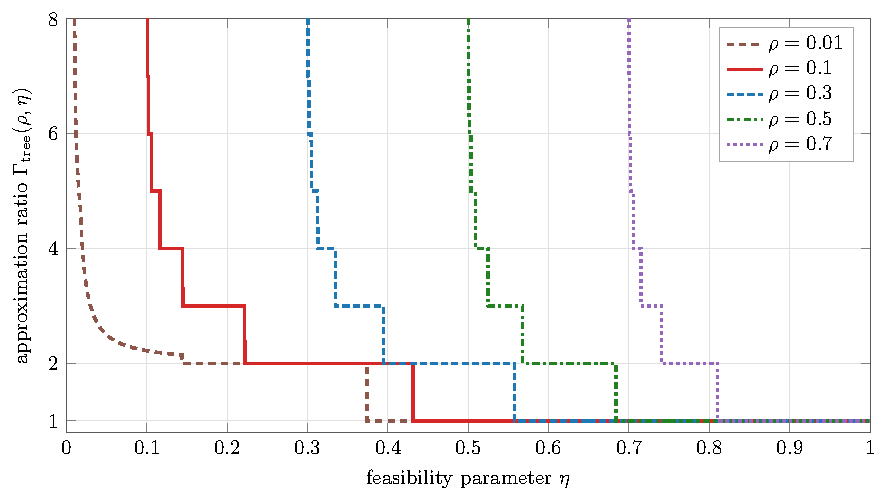
\includegraphics[width=0.92\textwidth]{figures/generated/tree_approximation_ratio_2d_plot.pdf}
  \caption{The combined approximation ratio from Corollary~\ref{cor:tree-best-bicriteria} as a function of $\eta$ for representative values of $\rho$. Values above $8$ are capped at $8$.}
  \label{fig:tree-approximation-ratio}
\end{figure}

        \begin{figure}[!tbp]
  \centering
  % Rendered on demand from tree_approximation_ratio_3d_plot.tex.
  % Keeping the dense PGFPlots surface as a PDF avoids rebuilding it with
  % every manuscript compilation.
  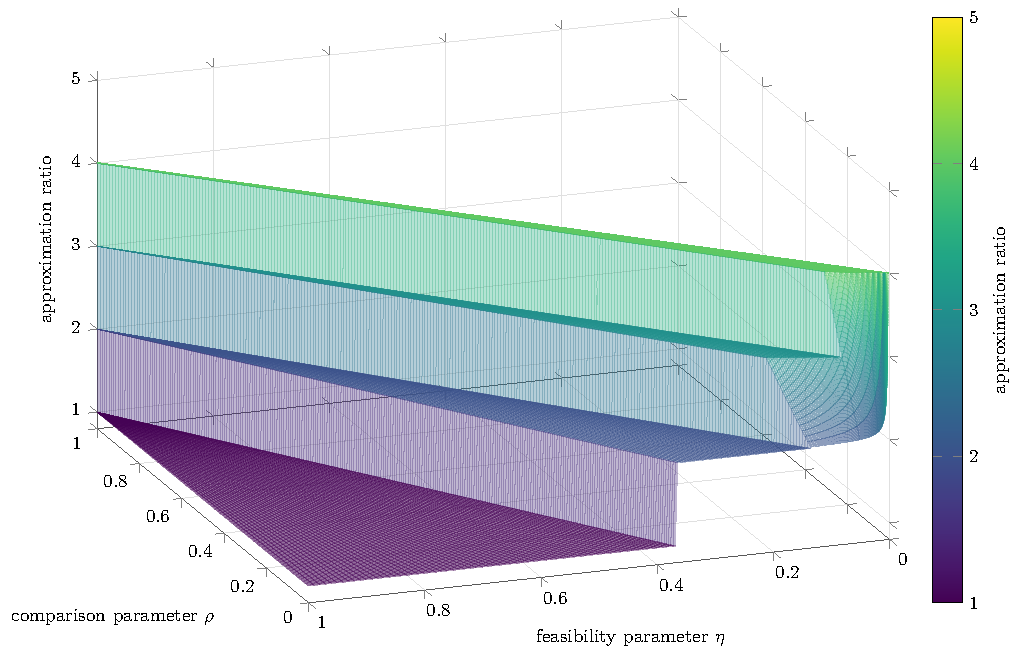
\includegraphics[width=0.94\textwidth]{figures/generated/tree_approximation_ratio_3d_plot.pdf}
  \caption{Combined tree approximation guarantee $\Gamma_{\mathrm{tree}}(\rho,\eta)$ from Corollary~\ref{cor:tree-best-bicriteria}, over $0<\rho<\eta<1$ (shown for $0.005\leq\rho\leq0.995$). Below the threshold, the height is the minimum of the anchored-LP, recursive, and hybrid bounds; above it, the direct dynamic program gives ratio $1$. Heights are capped at $12$. The plateaus reflect floor-log terms in the recursive and hybrid bounds.}
  \label{fig:tree-approximation-ratio-3d}
\end{figure}


        \subsection{Consequences for hierarchical clustering on trees}

        Combining Theorem~\ref{thm:tree-centroid-max-coverage} with Theorem~\ref{thm:hc-gpd-transfer} gives a $\frac{4e}{e-1}$-approximation for \textsc{Hierarchical Clustering with Demands} on trees.

        \begin{corollary}\label{cor:tree-hc-improved}
            There is a polynomial-time $\frac{4e}{e-1}$-approximation algorithm for \textsc{Hierarchical Clustering with Demands} on supply trees.
        \end{corollary}
        \begin{proof}
            Set $\rho=\frac12$ and $\eta=\frac{e+1}{2e}$. Then
            \[
                \frac{1-\rho}{\eta-\rho}=e,
                \qquad
                \Gamma_{\mathrm{MC}}(\rho,\eta)=\left\lceil\ln e\right\rceil=1.
            \]
            Theorem~\ref{thm:tree-centroid-max-coverage} therefore gives a polynomial-time subroutine with $\gamma(\eta)=1$. By Theorem~\ref{thm:hc-gpd-transfer}, the resulting approximation ratio is
            \[
                \frac{2}{1-\eta}=\frac{4e}{e-1}.
            \]
        \end{proof}


\section{Hardness of Graph Partitioning with Demands}\label{sec:gpd-hardness}

We next provide an approximation-hardness result for \textsc{Graph Partitioning with Demands} based on the Small-Set Expansion Hypothesis. The \emph{Small-Set Expansion Hypothesis} states that, for every constant $\zeta>0$, there is a constant $\delta>0$ for which it is NP-hard, given a regular graph, to distinguish between the existence of a vertex set of normalized size $\delta$ and expansion at most $\zeta$, and the condition that every vertex set of normalized size $\delta$ has expansion at least $1-\zeta$.

For the weighted graph $X$ in the reduction, define the normalized vertex measure
\[
    \mu(S)=\frac{\operatorname{vol}_X(S)}{\operatorname{vol}_X(U)}.
\]
Thus $\mu(U)=1$ and $\mu(u)$ is the stationary probability of stepping into $u$ under the random walk on $X$. Since multiplying all edge weights by the same constant changes neither expansion nor approximation ratios, we normalize $\operatorname{vol}_X(U)=1$. With this normalization, the expansion of a nonempty set $S$ is
\[
    \Phi_X(S)=\frac{c\br{S,U\setminus S}}{\mu(S)}.
\]

We also recall the Gaussian expansion profile used in the source theorem. For $r\in[0,1)$ and $\alpha\in(0,1)$, let
\[
    \begin{pmatrix}Z\\Z'\end{pmatrix}
    \sim\mathcal{N}\left(
        \begin{pmatrix}0\\0\end{pmatrix},
        \begin{pmatrix}1&r\\r&1\end{pmatrix}
    \right).
\]
Thus $Z$ and $Z'$ are standard Gaussian random variables with correlation $r$. Let $t_\alpha\in\mathbb{R}$ satisfy $\Pr[Z\geq t_\alpha]=\alpha$. We define the expansion profile of the Gaussian noise graph $\mathcal{G}(r)$ by
\[
    \Phi_{\mathcal{G}(r)}(\alpha)
    =\Pr\left[Z'<t_\alpha\mid Z\geq t_\alpha\right]
    =1-\frac{\Pr[Z\geq t_\alpha,\,Z'\geq t_\alpha]}{\alpha}.
\]

We first invoke the following result of Raghavendra, Steurer, and Tulsiani~\cite[Theorem~3.5]{ReductionsBetweenExpansionProblems}.

\begin{theorem}[Raghavendra-Steurer-Tulsiani]\label{thm:rst-global-expansion}
    For every integer $q\geq2$ and every $\varepsilon,\gamma>0$, assuming the Small-Set Expansion Hypothesis, it is hard to distinguish between the following cases for a weighted graph $X=(U,F,c)$:
    \begin{description}
        \item[YES:] There is a partition $\cP=\{S_1,\ldots,S_q\}$ of $U$ such that, for every $i\in[q]$, 
            $\mu(S_i)=\frac{1}{q}$ and $\Phi_X(S_i)\leq\varepsilon+o(\varepsilon)$.
        \item[NO:] Every $S\subseteq U$ satisfies $
            \Phi_X(S)
            \geq
            \Phi_{\mathcal{G}(1-\varepsilon/2)}(\mu(S))
            -\frac{\gamma}{\mu(S)}$.
    \end{description}
\end{theorem}

We derive from Theorem~\ref{thm:rst-global-expansion} the form of the gap used in our reduction.

\begin{lemma}\label{lem:globalized-long-code-gap}
    Fix an integer $q\geq2$ and a constant $b\in(0,1/2]$. Assuming the Small-Set Expansion Hypothesis, for every sufficiently small $\varepsilon>0$ it is hard to distinguish between the following cases for a weighted graph $X=(U,F,c)$:
    \begin{description}
        \item[YES:] There is a partition $\cP=\brc{S_1,\ldots,S_q}$ of $U$
        such that, for every $i\in[q]$, $
            \mu(S_i)=\frac{1}{q}$ and $
            \Phi_X(S_i)\leq K\cdot\varepsilon,$
        where $K>0$ is a universal constant.
        \item[NO:] For every $S\subseteq U$, where $b\leq\mu(S)\leq\frac{1}{2}$, $\Phi_X(S)\geq a_b\cdot \sqrt{\varepsilon},$
        where $a_b>0$ depends only on $b$.
    \end{description}
\end{lemma}
\begin{proof}
    In the YES case of Theorem~\ref{thm:rst-global-expansion}, the sets $S_1,\ldots,S_q$ have total measure $1$ and therefore form a partition of $U$. Moreover, $\varepsilon+o(\varepsilon)\leq K\cdot\varepsilon$ for a universal constant $K$ and all sufficiently small $\varepsilon$.

    Consider now the NO case. If $\alpha\in[b,1/2]$, then $t_\alpha$ ranges over a bounded interval depending only on $b$. The standard estimate for the probability that two highly correlated Gaussian variables lie on opposite sides of such a threshold gives $
        \Phi_{\mathcal{G}(1-\varepsilon/2)}(\alpha)
        \geq a'_b\cdot\sqrt{\varepsilon}$
    for some constant $a'_b>0$ and all sufficiently small $\varepsilon$. Indeed, the standard deviation of $Z'-Z$ is $\sqrt{\varepsilon}$, while the Gaussian density at $t_\alpha$ is bounded above and below by positive constants depending only on $b$. Taking $\gamma\leq b\cdot a'_b\cdot\sqrt{\varepsilon}/2$ yields
    \[
        \Phi_X(S)\geq\frac{a'_b}{2}\cdot\sqrt{\varepsilon}
    \]
    whenever $b\leq\mu(S)\leq1/2$. The claim follows with $a_b=a'_b/2$.
\end{proof}

\subsection{The reduction}

For simplicity, we carry out the reduction with rational weights. In order for the capacities and demands to be natural numbers, we may always multiply all of them by a common denominator. This does not affect feasibility or any approximation ratio, and hence does not affect the analysis.

A demand graph is \emph{bipartite multiplicative} if its vertex set has a bipartition $L\mathbin{\dot\cup}R$, its demand edges are all pairs with one endpoint in each side, and there is a potential $\pi$ such that $w(uv)=\pi(u)\cdot \pi(v)$ for every demand edge $uv$. Our intention is to show a reduction which establishes the hardness of graph partitioning with bipartite multiplicative demands.
This class is closed under taking induced subgraphs.


    For every $u\in U$, introduce two vertices $u^{\mathrm L}$ and $u^{\mathrm R}$, assign $
        \pi\br{u^{\mathrm L}}=\pi\br{u^{\mathrm R}}=\mu(u),$
    and let $
        \widetilde U
        =\brc{u^{\mathrm L},u^{\mathrm R}\colon u\in U}.$
    On $\widetilde U$, define the bipartite multiplicative demand graph to have edge set $
        D_\times
        =\brc{u^{\mathrm L}v^{\mathrm R}\colon u,v\in U\times U}$ and demands $
        w\br{u^{\mathrm L},v^{\mathrm R}}
        =\pi\br{u^{\mathrm L}}\cdot \pi\br{v^{\mathrm R}}.$
    For $S\subseteq U$, write $
        \widetilde S=\brc{u^{\mathrm L},u^{\mathrm R}\colon u\in S}.$
\begin{lemma}\label{lem:multiplicative-demands-encode-measure}
    For any $S\subseteq U$, we have, $
        {w\br{\widetilde S}}
        =\mu(S)^2$. In particular, $w\br{\widetilde U}=1$.
\end{lemma}
\begin{proof}
    Every pair $(u,v)\in S\times S$ indexes the unique demand edge $u^{\mathrm L}v^{\mathrm R}$. Therefore,
    \[
        w\br{\widetilde S}
        =\sum_{(u,v)\in S\times S}\pi\br{u^{\mathrm L}}\cdot \pi\br{v^{\mathrm R}}
        =\left(\sum_{u\in S}\mu(u)\right)^2
        =\mu(S)^2.
    \]
    The same calculation for $S=U$ gives $w\br{\widetilde U}=1$.
\end{proof}

We now turn $X$ into a supply graph $\widetilde X$ on $\widetilde U$. For every $uv\in F$, add the supply edge $u^{\mathrm L}v^{\mathrm L}$ with capacity $c(uv)$. For every $u\in U$, also add the \emph{consistency edge} $u^{\mathrm L}u^{\mathrm R}$ with capacity $1$. Thus, unless a consistency edge is cut, the two copies of every vertex belong to the same component. Together with the previously defined bipartite multiplicative demand graph on $\widetilde U$, this completes the construction of the instance $(\widetilde X,D_\times)$.

\subsection{Completeness}
\begin{lemma}\label{lem:sse-gpd-completeness}
    Fix $\rho\in(0,1)$ and set $
        q=\max\left\{2,\left\lceil\rho^{-1/2}\right\rceil\right\}. $
    In the YES case,
    \[
        \OPTdem{\widetilde X}{\rho}\leq \frac{K}{2}\cdot\varepsilon.
    \]
\end{lemma}
\begin{proof}
    For every $i\in[q]$, define $
        \widetilde S_i
        =\brc{u^{\mathrm L},u^{\mathrm R}\colon u\in S_i}.$
    Since $S_1,\ldots,S_q$ partition $U$, the sets $\widetilde S_1,\ldots,\widetilde S_q$ partition $\widetilde U$. Let $C_{\mathrm{yes}}$ consist of the supply edges $u^{\mathrm L}v^{\mathrm L}$ for which $uv\in F$ has endpoints in distinct parts of the original partition. Thus all consistency edges $u^{\mathrm L}u^{\mathrm R}$ are retained. Every crossing edge of $X$ is counted twice in the sum of the boundaries, and hence
    \[
        c\br{C_{\mathrm{yes}}}
        =\frac{1}{2}\sum_{i=1}^{q}c\br{S_i,U\setminus S_i}.
    \]
    By Lemma~\ref{lem:globalized-long-code-gap},
    \[
        c\br{C_{\mathrm{yes}}}
        \leq\frac{1}{2}\sum_{i=1}^{q}\mu(S_i)\cdot K\cdot\varepsilon
        =\frac{K\cdot\varepsilon}{2}.
    \]

    Every component $\widetilde H$ of $\widetilde X\setminus C_{\mathrm{yes}}$ is a union of left-right pairs corresponding to a set $H\subseteq S_i$ for some $i$. Therefore, by Lemma~\ref{lem:multiplicative-demands-encode-measure},
    \[
        \frac{w\br{\widetilde H}}{w\br{\widetilde U}}
        =\mu(H)^2
        \leq\mu(S_i)^2
        =\frac{1}{q^2}
        \leq\rho.
    \]
    Thus $C_{\mathrm{yes}}$ is $\rho$-feasible and has cost at most $\frac{K\cdot\varepsilon}{2}$.
\end{proof}

\subsection{Soundness}
We start by proving a numerical lemma that will be useful in the soundness analysis.
\begin{lemma}\label{lem:group-small-components}
    Let $p_1,\ldots,p_m\geq0$ satisfy $
        \sum_{i=1}^{m}p_i=1$ and $
        p_i\leq\sqrt{\eta}<1.$
    Define $b_\eta=\min\left\{\frac{1}{4},1-\sqrt{\eta}\right\}$.
    Then, there is a set $I\subseteq[m]$ such that
    \[
        b_\eta\leq\sum_{i\in I}p_i\leq\frac{1}{2}.
    \]
\end{lemma}
\begin{proof}
    If some $p_i>1/2$, take all indices except $i$. Their total is at least $1-\sqrt{\eta}\geq b_\eta$ and is less than $1/2$.
    Otherwise, we have $p_i\leq1/2$. If some $p_i\geq b_\eta$, take that index. If all $p_i<b_\eta$, add indices until their sum first reaches $b_\eta$. The resulting sum is less than $2b_\eta\leq1/2$.
\end{proof}

\begin{lemma}\label{lem:sse-gpd-soundness}
    In the NO case, every $\eta$-feasible supply-edge set $C$ satisfies $
        c\br{C}\geq\beta_\eta\cdot\sqrt{\varepsilon}
    $
    for some constant $\beta_\eta>0$ depending only on $\eta$, provided that $\varepsilon$ is sufficiently small.
\end{lemma}
\begin{proof}
    Set $\beta_\eta=b_\eta\cdot a_{b_\eta}$. We may assume that $\beta_\eta\cdot\sqrt{\varepsilon}\leq1$. If $C$ contains a consistency edge, then $c\br{C}\geq1\geq\beta_\eta\cdot\sqrt{\varepsilon}$, as required.

    Suppose now that no consistency edge is cut. Let $\widetilde H_1,\ldots,\widetilde H_m$ be the components of $\widetilde X\setminus C$. Every $\widetilde H_i$ is a union of left-right pairs. Let $H_i\subseteq U$ be their projection and put $p_i=\mu(H_i)$. The sets $H_1,\ldots,H_m$ partition $U$. By $\eta$-feasibility and Lemma~\ref{lem:multiplicative-demands-encode-measure},
    \[
        p_i^2 = \mu(H_i)^2
        =\frac{w\br{\widetilde H_i}}{w\br{\widetilde U}}
        \leq\eta,
    \]
    and hence $p_i\leq\sqrt{\eta}$. Apply Lemma~\ref{lem:group-small-components} and let $
        S=\bigcup_{i\in I}H_i.$
    Then $b_\eta\leq\mu(S)\leq1/2$. Every original-copy supply edge corresponding to an edge of $X$ crossing $\br{S,U\setminus S}$ joins two distinct components of $\widetilde X\setminus C$ and therefore belongs to $C$. Consequently, $
        c\br{C}\geq c\br{S,U\setminus S},
    $ so by Lemma~\ref{lem:globalized-long-code-gap},
    \[
        c\br{S,U\setminus S}
        =\mu(S)\cdot\Phi_X(S)
        \geq b_\eta\cdot a_{b_\eta}\sqrt{\varepsilon}
        =\beta_\eta\cdot\sqrt{\varepsilon}.
    \]
    which completes the proof.
\end{proof}
\subsection{Hardness of approximation}
\begin{theorem}\label{thm:sse-gpd-bicriteria-hardness}
    Fix constants $0<\rho<\eta<1$. Then, for any sufficiently small $\varepsilon>0$, a universal constant $L$ and a constant $\beta_\eta>0$ dependent only on $\eta$ such that it is SSEH-hard to distinguish between the following two cases:
    \begin{itemize}
        \item \textbf{YES case:} $\OPTdem{\widetilde X}{\rho}\leq L\cdot\varepsilon$.
        \item \textbf{NO case:} Every $\eta$-feasible supply-edge set $C$ satisfies $c\br{C}\geq\beta_\eta\cdot\sqrt{\varepsilon}$.
    \end{itemize}
    Consequently, assuming the Small-Set Expansion Hypothesis, for any constant $A>0$ there is no polynomial-time $(A,\eta)$-bicriteria approximation for \textsc{Graph Partitioning with Demands}, even for bipartite multiplicative demands.
\end{theorem}
\begin{proof}
    Let $L=\frac{K}{2}$. 
    In the YES case, Lemma~\ref{lem:sse-gpd-completeness} gives $\OPTdem{\widetilde X}{\rho}\leq L\cdot\varepsilon$. 
    In the NO case, Lemma~\ref{lem:sse-gpd-soundness} says that every $\eta$-feasible cut has cost at least $\beta_\eta\cdot\sqrt{\varepsilon}$. 
    Now, suppose that such an algorithm exists. Choose $\varepsilon>0$ sufficiently small that all preceding statements apply and
    \[
        A\cdot L\cdot\varepsilon<\beta_\eta\cdot\sqrt{\varepsilon}.
    \]
    Equivalently, it is enough to take
    \[
        \varepsilon<\left(\frac{\beta_\eta}{A\cdot L}\right)^2.
    \]
    Thus the algorithm distinguishes the YES and NO instances of Lemma~\ref{lem:globalized-long-code-gap}, contradicting the Small-Set Expansion Hypothesis.
\end{proof}

The hardness also transfers to the \textsc{Generalized Conductance} problem, as formalized in the following corollary.

\begin{corollary}\label{cor:sse-generalized-conductance-hardness}
    It is SSEH-hard to approximate \textsc{Generalized Conductance} within any constant factor, even for bipartite multiplicative demands.
\end{corollary}
\begin{proof}
    Theorem~\ref{thm:gpd-extension} certifies that a constant-factor approximation for \textsc{Generalized Conductance} would yield a constant-factor bicriteria approximation for \textsc{Graph Partitioning with Demands}, contradicting Theorem~\ref{thm:sse-gpd-bicriteria-hardness}.
\end{proof}

\section{Conclusions}

We introduced and studied the \textsc{Generalized Conductance}, a problem of interest on its own, and also important from the perspective of potential applications. Our algorithms yield an $\bigo\br{\sqrt{\log n}}$-approximation on general graphs through a reduction to \textsc{Min-Ratio Vertex Cut}, and an exact algorithm on supply trees.

Beyond the core objective, we showed that these approximation ratios carry over to natural downstream tasks. In particular, we obtained an $\bigo\br{\sqrt{\log n}}$ bicriteria approximation for \textsc{Graph Partitioning with Demands} and an $\bigo\br{\sqrt{\log n}}$-approximation for \textsc{Hierarchical Clustering with Demands}, with a corresponding $\bigo\br{1}$-approximation for trees. For \textsc{Graph Partitioning with Demands} on supply trees, we developed a two-separator recursion using submodular maximum coverage, together with a full-quota $(4+\epsilon)$-approximation whose polynomial degree depends on $1/\rho$. These guarantees complement the anchored-LP and weighted-budget approaches. It is of interest whether our algorithms apply to other tasks in the presence of demands, such as network design or routing.

One may consider generalizing our setup to the case when both cost and demand functions are given on arbitrary hypergraphs. Here, a similar situation occurs since few approximation algorithms for \textsc{Hypergraph Sparsest Cut} are known \cite{DiversityEmbeddingsAndTheHypergraphSparsestCut,BoundsOnTheMaxFlowMinCutRatioForDirectedMulticommodityFlows}, but we are not aware of any results on hypergraph analogues of other graph partitoning objectives studied in this work. What would probably be required in order to tackle these tasks is a new notion of hypergraph conductance, similar in spirit to our generalized conductance. Obtaining approximation algorithms for such a measure would be an interesting direction for future work.

Incorporating our setup into the framework of spectral graph theory is another promising direction. In particular, it is known that the classical conductance is closely related to the second eigenvalue of the Laplacian matrix of a graph. It would be of interest to see whether a similar relationship can be established for generalized conductance and some appropriate generalization of the Laplacian matrix.



\bibliography{references}

\end{document}
